We now investigate inductive types with propositional computation rules in the setting of homotopy type theory. We start by revisiting the type $\Bool$ of Boolean truth values.

\subsection{The type $\Bool$}
Although the rules for the type $\Bool$ as presented in section \ref{subsection:bool} are the natural ones to consider in the setting of homotopy type theory, they do not imply a strict universal property. For example, given a type $C:\UU_i$ and elements $c_0, c_1 : C$, the function $\lam{x:\Bool}\boolrec(C,c_0,c_1,x) : \Bool \rightarrow C$ cannot, in general, be shown to be definitionally unique among the functions $f : \Bool \rightarrow C$ with the property that $f(0) \equiv c_0 : C$ and $f(1) \equiv c_1 : C$.\ednote{Do we need a reference for this?}
The best that one can do is to show that it is unique among all such maps up to a path, which itself is unique up to a higher path, which in turn is unique up to a yet higher path, etc. This sort of ``homotopy" $\omega$-universality, which apparently involves infinitely much data, can nonetheless be captured directly within the system of type theory (without resorting to coinduction) using ideas from higher category theory. To obtain a full characterization of the type $\Bool$ using this alternate universal condition, we relax the computation rules from section \ref{subsection:bool} to involve propositional, rather than definitional, equality: \smallskip
\begin{itemize}
\item Propositional $\Bool$-computation rules. \smallskip
\begin{equation*}
\begin{prooftree}
x:\Bool \vdash E(x) : \UU_i \qquad
e_0 : E(0) \qquad
e_1 : E(1)
\justifies
\left\{
\begin{array}{c} 
 \boolindcompo_{\UU_i}(x.E,e_0,e_1) : \boolind(0)  =  e_0  \, , \\
 \boolindcompi_{\UU_i}(x.E,e_0,e_1) : \boolind(1)  =  e_1 \, .
 \end{array}
\right.
\end{prooftree}
 \end{equation*}
\item Simple propositional $\Bool$-computation rules. \smallskip 
\begin{equation*}
\begin{prooftree}
C : \UU_i \qquad
c_0 : C \qquad
c_1 : C \qquad
b : \Bool
\justifies
\left\{
\begin{array}{c} 
 \boolreccompo_{\UU_i}(C,c_0,c_1) : \boolrec(0)  =  c_0  \, , \\
 \boolreccompi_{\UU_i}(C,c_0,c_1) : \boolrec(1)  =  c_1 \, .
 \end{array}
\right.
\end{prooftree}
 \end{equation*} 
\end{itemize} \smallskip
As discussed above, the uniqueness principles can still be shown to hold, albeit in a propositional form: \smallskip

\begin{itemize}
\item Propositional $\Bool$-uniqueness principle.\smallskip
\begin{mathpar}
\inferrule{b : \Bool \\ x : \Bool \vdash E(x) : \UU_i \\ e_0 : E(0) \\ e_1 : E(1) \\ \\\\ x : \Bool \vdash f(x) : E(x) \\ \gamma_0 : f(0) = e_0 \\ \gamma_1 : f(1) = e_1 \\ \\\\ x : \Bool \vdash g(x) : E(x) \\ \delta_0 : g(0) = e_0 \\ \delta_1 : g(1) = e_1}{\boolinduniq_{\UU_i}(x.E, e_0, e_1, x.f, \gamma_0, \gamma_1, x.g, \delta_0, \delta_1, b) : f(b) = g(b)}
\end{mathpar}
\item Simple propositional $\Bool$-uniqueness principle.\smallskip
\begin{mathpar}
\inferrule{b : \Bool \\ C : \UU_i \\ c_0 : C \\ c_1 : C \\ \\\\ x : \Bool \vdash f(x) : C \\ \gamma_0 : f(0) = c_0 \\ \gamma_1 : f(1) \equiv c_1 \\ \\\\ x : \Bool \vdash g(x) : C \\ \delta_0 : g(0) = c_0 \\ \delta_1 : g(1) = c_1}{\boolrecuniq_{\UU_i}(C, c_0, c_1, x.f, \gamma_0, \gamma_1, x.g, \delta_0, \delta_1, b) : f(b) = g(b)}
\end{mathpar}
\end{itemize} \smallskip
The witness terms will be shortened to $\boolinduniq(b)$, $\boolrecuniq(b)$ where appropriate. In showing the above laws, we proceed analogously to the extensional case: we use the induction principle with the type family $x \mapsto f(x) =_{E(x)} g(x)$ and for the cases $x \defeq 0$, $x \defeq 1$ we supply the paths $\gamma_0 \ct \delta_0^{-1}$ and $\gamma_1 \ct \delta_1^{-1}$ respectively. This gives us a pointwise propositional equality between $f$ and $g$ as desired. The simple uniqueness principle follows at once from the dependent one.

Unlike in the extensional setting, however, $\boolinduniq(b)$ will generally not be an identity path. The natural question to ask is how $\boolinduniq(-)$ behaves on the constructors $0$, $1$. Since $\boolinduniq(b)$ was constructed using the $\Bool$-induction principle, we invoke the corresponding (propositional) computation rules to get the following coherence rules:\smallskip
\begin{itemize}
\item Propositional $\Bool$-coherence principles.\smallskip
\begin{equation*}
\begin{prooftree}
\begin{array}{ccc} 
 x : \Bool \vdash E(x) : \UU_i & e_0 : E(0) & e_1 : E(1) \\
 x : \Bool \vdash f(x) : E(x) \;\;\;\;\;\; & \gamma_0 : f(0) = e_0 \;\;\;\;\;\; & \gamma_1 : f(1) = e_1 \\
 x : \Bool \vdash g(x) : E(x) \;\;\;\;\;\; & \delta_0 : g(0) = e_0 \;\;\;\;\;\; & \delta_1 : g(1) = e_1 \\
\end{array}
\justifies
\left\{
\begin{array}{c} 
 \boolindcoho_{\UU_i}(x.E, e_0, e_1, x.f, \gamma_0, \gamma_1, x.g, \delta_0, \delta_1) : \boolinduniq(0) = \gamma_0 \ct \delta_0^{-1}  \, , \\
 \boolindcohi_{\UU_i}(x.E, e_0, e_1, x.f, \gamma_0, \gamma_1, x.g, \delta_0, \delta_1) : \boolinduniq(1) = \gamma_1 \ct \delta_1^{-1} \, .
 \end{array}
\right.
\end{prooftree}
\end{equation*}
\item Simple propositional $\Bool$-coherence principles.\smallskip
\begin{equation*}
\begin{prooftree}
\begin{array}{ccc} 
 C : \UU_i & c_0 : C & c_1 : C \\
 x : \Bool \vdash f(x) : C \;\;\;\;\;\; & \gamma_0 : f(0) = c_0 \;\;\;\;\;\; & \gamma_1 : f(1) = c_1 \\
 x : \Bool \vdash g(x) : C \;\;\;\;\;\; & \delta_0 : g(0) = c_0 \;\;\;\;\;\; & \delta_1 : g(1) = c_1 \\
\end{array}
\justifies
\left\{
\begin{array}{c} 
 \boolreccoho_{\UU_i}(C, c_0, c_1, x.f, \gamma_0, \gamma_1, x.g, \delta_0, \delta_1) : \boolrecuniq(0) = \gamma_0 \ct \delta_0^{-1}  \, , \\
 \boolreccohi_{\UU_i}(C, c_0, c_1, x.f, \gamma_0, \gamma_1, x.g, \delta_0, \delta_1) : \boolrecuniq(1) = \gamma_1 \ct \delta_1^{-1} \, .
 \end{array}
\right.
\end{prooftree}
 \end{equation*} 
\end{itemize} \smallskip
This motivates the following definitions.
\begin{definition}\label{def:BoolCell}
For $\X : \BoolAlg_{\UU_i}$, $\Y : \BoolAlg_{\UU_j}$ and homomorphisms $\mu, \nu : \BoolHom \; \X \; \Y$, define the type of \emph{2-cells} between $\mu$ and $\nu$ by
\begin{align*} & \BoolCell \; (C,c_0,c_1) \; (D, d_0 \; d_1) \; (f,\gamma_0,\gamma_1) \; (g,\delta_0,\delta_1) \defeq \\ & \;\;\; \;\;\;\BoolFibHom \; (C,c_0,c_1) \; (f \sim g, \gamma_0 \ct \delta_0^{-1}, \gamma_1 \ct \delta_1^{-1})
\end{align*}
\end{definition}

\begin{definition}\label{def:BoolFibCell}
For $\X : \BoolAlg_{\UU_i}$, $\Y : \BoolFibAlg_{\UU_j} \; \X$ and fibered homomorphisms $\mu, \nu : \BoolFibHom \; \X \; \Y$, define the type of \emph{fibered 2-cells} between $\mu$ and $\nu$ by
\begin{align*} & \BoolFibCell \; (C,c_0,c_1) \; (E, e_0 \; e_1) \; (f,\gamma_0,\gamma_1) \; (g,\delta_0,\delta_1) \defeq \\ & \;\;\; \;\;\;\BoolFibHom \; (C,c_0,c_1) \; (f \sim g, \gamma_0 \ct \delta_0^{-1}, \gamma_1 \ct \delta_1^{-1})
\end{align*}
\end{definition}
For brevity, we will often leave out the first two arguments.

We also need to update some of our previous terminology: it is a misnomer to call an algebra $\X$ \emph{initial} if the type of homomorphisms from $\X$ to any other algebra $\Y$ is contractible, since a contractible type may contain more than one element. Instead, an algebra with this property will be called \emph{homotopy-initial}; by Lem.~\ref{lem:contr_path_space} the contractibility requirement exactly captures the notion that there exists a homomorphism which is unique up to a path, which itself is unique up to a higher path, and so on. 

\begin{definition}\label{def:BoolHInit}
An algebra $\X : \BoolAlg_{\UU_i}$ is \emph{homotopy-initial} on a universe $\UU_j$ if for any algebra $\Y : \BoolAlg_{\UU_j}$, the type of $\Bool$-homomorphisms between $\X$ and $\Y$ is contractible:
\[ \IsBoolHInit_{\UU_j}(\X) \defeq \prd{(\Y:\BoolAlg_{\UU_j})} \iscontr(\BoolHom \; \X \; \Y) \]  
\end{definition}

In certain respects, algebras and algebra homomorphisms behave much like objects and morphisms in a category:
\begin{definition}
For any $\X : \BoolAlg_{\UU_i}$ there is a designated \emph{identity} homomorphism from $\X$ to itself, defined by
\[ \BoolIdHom \; (C,c_0,c_1) \defeq (\idfun{C}, \refl(c_0), \refl(c_1)) \]
\end{definition}
We often denote this homomorphism by $\one_\X$.

\begin{definition}
For algebras $\X : \BoolAlg_{\UU_i}$, $\Y : \BoolAlg_{\UU_j}$, $\Z : \BoolAlg_{\UU_k}$ and homomorphisms $\mu : \BoolHom \; \X \; \Y$, $\nu : \BoolHom \; \Y \; \Z$, the \emph{composition} of $\mu$ and $\nu$ is a homomorphism from $\X$ to $\Z$ defined by
\begin{align*} & \BoolCompHom \; (C,c_0,c_1) \; (D,d_0,d_1) \; (E,e_0,e_1) \; (f,\gamma_0,\gamma_1) \; (g,\delta_0,\delta_1) \defeq \\ & \;\;\;\;\;\; \big(g \comp f, g(\gamma_0) \ct \delta_0, g(\gamma_1) \ct \delta_1\big)
\end{align*}
\end{definition}
We often leave out the first three arguments and denote the composition by $\nu \comp \mu$.

\begin{definition}
For $\X : \BoolAlg_{\UU_i}$, $\Y : \BoolAlg_{\UU_j}$ we define the type of \emph{isomorphisms} between $\X$ and $\Y$ as
\[\BoolAlgIso \; \X \; \Y \defeq \sm{(\rho : \BoolHom \; \X \; \Y)} \Big( \sm{(\mu : \BoolHom \; \Y \; \X)} \mu \comp \rho = \one_\X \Big) \times \Big( \sm{(\nu : \BoolHom \; \Y \; \X)} \rho \comp \nu = \one_\Y \Big) \] 
\end{definition}

\begin{lemma}\label{BoolFibHomSpace}
For $\X : \BoolAlg_{\UU_i}$, $\Y : \BoolFibAlg_{\UU_j} \; \X$ and $\mu,\nu : \BoolFibHom \; \X \; \Y$, the path space $\mu = \nu$ is equivalent to the space of fibered 2-cells between $\mu$ and $\nu$:
\[ \mu = \nu \;\; \simeq \;\; \BoolFibCell \; \mu \; \nu \] 
\end{lemma}
\begin{proof}
Let algebras $(C,c_0,c_1) : \BoolAlg_{\UU_i}$, $(E,e_0,e_1) : \BoolFibAlg_{\UU_j} \; (C,c_0,c_1)$ and homomorphisms $(f,\gamma_0,\gamma_1), (g,\delta_0,\delta_1) : \BoolFibHom \; (C,c_0,c_1) \; (E,e_0,e_1)$ be given. We have
\begin{alignat*}{4}
& (f,\gamma_0,\gamma_1) = (g,\delta_0,\delta_1) & \simeq \\
& \sm{\alpha : f = g} \Big((\gamma_0,\gamma_1) = \trans^{-1}_{h \mapsto h(c_0) = d_0 \times h(c_1) = d_1}(\alpha) \; (\delta_0,\delta_1) \Big) & \simeq \\
& \sm{\alpha : f = g} \Big((\gamma_0,\gamma_1) = \big(\happly(\alpha,c_0) \ct \delta_0, \happly(\alpha,c_1) \ct \delta_1\big) \Big) & \simeq \\
& \sm{\alpha : f = g} \Big(\gamma_0 = \happly(\alpha,c_0) \ct \delta_0\Big) \times \Big( \gamma_1 = \happly(\alpha,c_1) \ct \delta_1 \Big) & \;\;\; \simeq \\
& \sm{\alpha : f \sim g} \Big(\gamma_0 = \alpha(c_0) \ct \delta_0\Big) \times \Big(\gamma_1 = \alpha(c_1) \ct \delta_1 \Big) & \simeq \\
& \sm{\alpha : f \sim g} \Big(\alpha(c_0) = \gamma_0 \ct \delta^{-1}_0\Big) \times \Big(\alpha(c_1) = \gamma_1 \ct \delta^{-1}_1 \Big) & \equiv \\
& \BoolFibCell \; (f,\gamma_0,\gamma_1) \; (g,\delta_0,\delta_1)
\end{alignat*}
\end{proof}

\begin{corollary}\label{BoolHomSpace}
For $\X : \BoolAlg_{\UU_i}$, $\Y : \BoolAlg_{\UU_j}$ and $\mu,\nu : \BoolHom \; \X \; \Y$, the path space $\mu = \nu$ is equivalent to the space of 2-cells between $\mu$ and $\nu$:
\[ \mu = \nu \;\; \simeq \;\; \BoolCell \; \mu \; \nu \] 
\end{corollary}

\begin{lemma}\label{BoolAlgSpace}
For $\X,\Y : \BoolAlg_{\UU_i}$, the path space $\X = \Y$ is equivalent to the space of isomorphisms between $\X$ and $\Y$:
\[ \X = \Y \;\; \simeq \;\; \BoolAlgIso \; \X \; \Y \] 
\end{lemma}
\begin{proof}
Let algebras $(C,c_0,c_1), (D,d_0,d_1) : \BoolAlg_{\UU_i}$ be given. We have
\begin{alignat*}{4}
& \BoolAlgIso \; (C,c_0,c_1) \; (D,d_0,d_1) & \equiv \\
& \sm{\rho : \big(\sm{f:C\to D} f(c_0) =d_0 \times f(c_1) = d_1\big)} \Big(\sm{\mu : \big(\sm{g:D\to C} g(d_0)=c_0 \times g(d_1)=c_1\big)} \mu \comp \rho = \one_{(C,c_0,c_1)} \Big)\; \times & \\
& \;\;\;\;\;\;\;\;\;\;\;\;\;\;\;\;\;\;\;\;\;\;\;\;\;\;\;\;\;\;\;\;\;\;\;\;\;\;\;\;\;\;\;\;\;\Big(\sm{\nu : \big(\sm{h:D\to C} h(d_0)=c_0 \times g(d_1)=c_1\big)} \rho \comp \nu = \one_{(D,d_0,d_1)}\Big) & \;\;\;\;\;\;\; \simeq \\
& \sm{f : C\to D} \sm{\epsilon_0 : f(c_0)=d_0} \sm{\epsilon_1 : f(c_1) = d_1} \Big(\sm{g:D\to C} \sm{\gamma_0 : g(d_0)=c_0} \sm{\gamma_1 : g(d_1) = c_1} P_{f,\epsilon_0,\epsilon_1,g,\gamma_0,\gamma_1}\Big) \; \times & \\
& \;\;\;\;\;\;\;\;\;\;\;\;\;\;\;\;\;\;\;\;\;\;\;\;\;\;\;\;\;\;\;\;\;\;\;\;\;\;\;\;\;\;\;\;\;\;\;\;\; \Big(\sm{h:D\to C} \sm{\delta_0 : h(d_0)=c_0} \sm{\delta_1 : h(d_1) = c_1} Q_{f,\epsilon_0,\epsilon_1,h,\delta_0,\delta_1} \Big) &
\end{alignat*}
where
\begin{align*}
& P_{f,\epsilon_0,\epsilon_1,g,\gamma_0,\gamma_1} \defeq \Big(g \comp f, \app_g(\epsilon_0) \ct \gamma_0, \app_g(\epsilon_1) \ct \gamma_1\Big) = \Big(\idfun{C}, \refl_{c_0}, \refl_{c_1}\Big) \\
& Q_{f,\epsilon_0,\epsilon_1,h,\delta_0,\delta_1} \defeq \Big(f \comp h, \app_f(\delta_0) \ct \epsilon_0, \app_f(\delta_1) \ct \epsilon_1\Big) = \Big(\idfun{D}, \refl_{d_0}, \refl_{d_1}\Big)
\end{align*}
Now we have
\begin{alignat*}{4}
& P_{f,\epsilon_0,\epsilon_1,g,\gamma_0,\gamma_1} & \equiv \\
& \Big(g \comp f, \app_g(\epsilon_0) \ct \gamma_0, \app_g(\epsilon_1) \ct \gamma_1\Big) = \Big(\idfun{C}, \refl_{c_0}, \refl_{c_1}\Big) & \simeq \\
& \sm{\alpha : g \comp f = \idfun{C}} \Big(\app_g(\epsilon_0) \ct \gamma_0, \app_g(\epsilon_1) \ct \gamma_1\Big) = \trans^{-1}_{i \mapsto i(c_0) = c_0 \times i(c_1) = c_1}(\alpha) \; \Big(\refl_{c_0}, \refl_{c_1}\Big) & \;\;\; \simeq \\
& \sm{\alpha : g \comp f = \idfun{C}} \Big(\app_g(\epsilon_0) \ct \gamma_0, \app_g(\epsilon_1) \ct \gamma_1\Big) = \Big(\happly(\alpha,c_0) \ct \refl_{c_0}, \happly(\alpha,c_1) \ct \refl_{c_1}\Big) & \;\;\; \simeq \\
& \sm{\alpha : g \comp f = \idfun{C}} \Big(\app_g(\epsilon_0) \ct \gamma_0 = \happly(\alpha,c_0) \ct \refl_{c_0}\Big) \times \Big(\app_g(\epsilon_1) \ct \gamma_1 = \happly(\alpha,c_1) \ct \refl_{c_1}\Big) & \;\;\; \simeq \\
& \sm{\alpha : g \comp f \sim \idfun{C}} \Big(\app_g(\epsilon_0) \ct \gamma_0 = \alpha(c_0) \ct \refl_{c_0}\Big) \times \Big(\app_g(\epsilon_1) \ct \gamma_1 = \alpha(c_1) \ct \refl_{c_1}\Big) & \;\;\; \simeq \\
& \sm{\alpha : g \comp f \sim \idfun{C}} \Big(\alpha(c_0) = \app_g(\epsilon_0) \ct \gamma_0 \Big) \times \Big(\alpha(c_1) = \app_g(\epsilon_1) \ct \gamma_1\Big) &
\end{alignat*}
and analogously
\begin{alignat*}{4}
Q_{f,\epsilon_0,\epsilon_1,h,\delta_0,\delta_1} \simeq \sm{\beta : f \comp h \sim \idfun{D}} \Big(\beta(d_0) = \app_f(\delta_0) \ct \epsilon_0 \Big) \times \Big(\beta(d_1) = \app_f(\delta_1) \ct \epsilon_1\Big)
\end{alignat*}
Thus we can express $\BoolAlgIso \; (C,c_0,c_1) \; (D,d_0,d_1)$ equivalently as the type
\begin{alignat*}{4}
& \sm{f : C\to D} \sm{\epsilon_0 : f(c_0)=d_0} \sm{\epsilon_1 : f(c_1) = d_1} \sm{g:D\to C} \sm{\alpha : g \comp f \sim \idfun{C}} \sm{h:D \to C} \sm{\beta : f \comp h \sim \idfun{D}} & \\
& \Big(\sm{\gamma_0 : g(d_0)=c_0} \alpha(c_0) = \app_g(\epsilon_0) \ct \gamma_0 \Big) \times \Big(\sm{\gamma_1 : g(d_1)=c_1} \alpha(c_1) = \app_g(\epsilon_1) \ct \gamma_1 \Big) \; \times & \\
& \Big(\sm{\delta_0 : h(d_0)=c_0} \beta(d_0) = \app_f(\delta_0) \ct \epsilon_0\Big) \times \Big(\sm{\delta_1 : h(d_1)=c_1} \beta(d_1) = \app_f(\delta_1) \ct \epsilon_1\Big) &
\end{alignat*}
Now we have
\[ \sm{\gamma_0 : g(d_0)=c_0} \Big(\alpha(c_0) = \app_g(\epsilon_0) \ct \gamma_0\Big) \;\;\; \simeq \;\;\; \sm{\gamma_0 : g(d_0)=c_0} \Big(\gamma_0 = \app_g(\epsilon_0)^{-1} \ct \alpha(c_0)\Big) \;\;\; \simeq \;\;\; \one\]
by Lem.~\ref{lem_singl_contr}\ednote{Which says $\iscontr(\sm{x:A} x = y)$}. Similarly, $\sm{\gamma_1 : g(d_1)=c_1} \Big(\alpha(c_1) = \app_g(\epsilon_1) \ct \gamma_1\Big)$ is equivalent to $\one$. We also have
\[ \sm{\delta_0 : h(d_0)=c_0} \Big(\beta(d_0) = \app_f(\delta_0) \ct \epsilon_0\Big) \;\;\; \simeq \;\;\; \sm{\delta_0 : h(d_0)=c_0} \Big(\app_f(\delta_0) = \beta(d_0) \ct \epsilon^{-1}_0\Big) \;\;\; \simeq \;\;\; \one \]
by Lem.~\ref{lem_singl_equiv_contr}\ednote{Which says $\iscontr(\sm{x:A} f(x) =_B y)$ if $f : A \to B$ is an equivalence},~\ref{lem_ap_equiv}\ednote{Which says $\app_f : x =_A y \to f(x) =_B f(y)$ is equivalence if $f : A \to B$ is}, and the fact that $g,\alpha,h,\beta$ make $f$ into an equivalence. Similarly, $\sm{\delta_1 : h(d_1)=c_1} \Big(\beta(d_1) = \app_f(\delta_1) \ct \epsilon_1\Big)$ is equivalent to $\one$. Thus, we have
\begin{alignat*}{4}
& \BoolAlgIso \; (C,c_0,c_1) \; (D,d_0,d_1) & \simeq \\
& \sm{f : C\to D} \sm{g:D\to C} \sm{\alpha : g \comp f \sim \idfun{C}} \sm{h:D \to C} \sm{\beta : f \comp h \sim \idfun{D}} \Big(f(c_0)=d_0\Big) \times \Big(f(c_1) = d_1\Big) & \;\;\; \simeq \\
& \sm{f : C\to D} \isequiv(f) \times \Big(f(c_0)=d_0\Big) \times \Big(f(c_1) = d_1\Big) & \;\;\; \simeq \\
& \sm{p : C \simeq D} \Big(\fst(p) \; c_0 =d_0\Big) \times \Big(\fst(p) \; c_1 = d_1\Big) & \;\;\; \simeq \\
& \sm{p : C \simeq D} \Big(\fst(p) \; c_0, \fst(p) \; c_1\Big) = (d_0, d_1) & \;\;\; \simeq \\
& \sm{p : C = D} \Big(\fst(\idtoeq(p)) \; c_0, \fst(\idtoeq(p)) \; c_1\Big) = (d_0, d_1) & \;\;\; \simeq \\
& \sm{p : C = D} \Big(\trans_{X \mapsto X \times X}(p) \; (c_0,c_1) = (d_0,d_1)\Big) & \simeq \\ 
& (C,c_0,c_1) = (D,d_0,d_1)
\end{alignat*}
\end{proof}

As desired, the analogues of the lemmas from section \ref{subsection:bool} still hold in the setting of homotopy type theory:

\begin{lemma}\label{lem:BoolIndImpUniqInt}
In $\Hint$, if an algebra $\X : \BoolAlg_{\UU_i}$ satisfies the induction principle on the universe $\UU_j$, it also satisfies the induction uniqueness principle on $\UU_j$. In other words, we have
\[ \HasBoolInd_{\UU_j}(\X) \;\; \rightarrow \;\; \HasBoolIndUniq_{\UU_j}(\X) \]
\end{lemma}
\begin{proof}
Let an algebra $(C,c_0,c_1) : \BoolAlg_{\UU_i}$ be given. To prove the induction uniqueness principle, take any algebra $(E,e_0,e_1) : \BoolFibAlg_{\UU_j} \; (C,c_0,c_1)$ and homomorphisms $(f,\gamma_0, \gamma_1), (g,\delta_0,\delta_1) : \BoolFibHom \; (C,c_0,c_1) \; (E,e_0,e_1)$. By Lem.~\ref{BoolFibHomSpace}, to show $(f,\gamma_0,\gamma_1) = (g,\delta_0,\delta_1)$ it suffices to exhibit a fibered 2-cell between $(f,\gamma_0,\gamma_1)$ and $(g,\delta_0,\delta_1)$. For this we use the induction principle with the fibered algebra $\big(f \sim g, \gamma_0 \ct \delta_0^{-1}, \gamma_1 \ct \delta_1^{-1}\big)$ and we are done.
\end{proof}

%\begin{lemma}\label{lem:BoolRecUniqEqInitInt}
%In $\Hint$, the following conditions on an algebra $\X : \BoolAlg_{\UU_i}$ are equivalent:
%\begin{enumerate}
%\item $\X$ satisfies the recursion and recursion uniqueness principles on the universe $\UU_j$
%\item $\X$ is homotopy-initial on the universe $\UU_j$
%\end{enumerate}
%In other words, we have
%\[ \HasBoolRec_{\UU_j}(\X) \times \HasBoolRecUniq_{\UU_j}(\X) \;\; \simeq \;\; \IsBoolHInit_{\UU_j}(\X) \]
%\end{lemma}
%\begin{proof}
%By Lem.~\ref{lem:ContrChar}.
%\end{proof}

\begin{corollary}
In $\Hint$, if an algebra $\X : \BoolAlg_{\UU_i}$ satisfies the induction principle on the universe $\UU_j$, it is homotopy-initial on $\UU_j$. In other words, we have
\[ \HasBoolInd_{\UU_j}(\X) \;\; \rightarrow \;\; \IsBoolHInit_{\UU_j}(\X) \]
\end{corollary}

\begin{lemma}\label{lem:BoolRecUniqImpIndInt}
In $\Hint$, if an algebra $\X : \BoolAlg_{\UU_i}$ satisfies the recursion and recursion uniqueness principles on the universe $\UU_j$ and $j \geq i$, then it satisfies the induction principle on $\UU_j$. In other words, we have
\[ \HasBoolRec_{\UU_j}(\X) \times \HasBoolRecUniq_{\UU_j}(\X) \;\; \rightarrow \; \; \HasBoolInd_{\UU_j}(\X) \]
provided $j \geq i$.
\end{lemma}
\begin{proof}
Let algebras $(C,c_0,c_1) : \BoolAlg_{\UU_i}$ and $(E,e_0,e_1) : \BoolFibAlg_{\UU_j} \; (C,c_0,c_1)$ be given. 
We use the recursion principle with the algebra $\big(\sm{x:C} E(x), (c_0,e_0), (c_1,e_1)\big)$. We note that the carrier type belongs to $\UU_j$ as $i \leq j$. This gives us a homomorphism $(u,\theta_0,\theta_1)$, where $u : C \to \sm{x:C} E(x)$, $\theta_0 : u(c_0) = (c_0,e_0)$, and $\theta_1 : u(c_1) = (c_1,e_1)$. We can now form two homomorphisms 
\[\Big(\fst \comp u, \fst(\idtodpair(\theta_0)), \fst(\idtodpair(\theta_1))\Big), \Big(\idfun{C}, \refl_{c_0}, \refl_{c_1}\Big) : \BoolHom \; (C,c_0,c_1) \; (C,c_0,c_1)\]
The recursion uniqueness principle tells us that these homomorphisms are equal. By Cor.~\ref{BoolHomSpace} this means there exists a 2-cell $(\alpha,\eta_0,\eta_1)$ between them, i.e., we have 
\begin{align*}
& \alpha : \fst \comp u \sim \idfun{C} \\
& \eta_0 : \alpha(c_0) = \fst(\idtodpair(\theta_0)) \ct \refl_{c_0} \\
& \eta_1 : \alpha(c_1) = \fst(\idtodpair(\theta_1)) \ct \refl_{c_1}
\end{align*}
We can thus define the desired fibered homomorphism as \[\Big(x \mapsto \trans_E(\alpha(x)) \; \snd(u(x)), \phi_0, \phi_1\Big) : \BoolFibHom \; (C,c_0,c_1) \; (E,e_0,e_1)\]
where $\phi_0$ is the path
\begin{center}
\begin{tikzpicture}
\node (N0) at (0,3) {$\trans_E\big(\alpha(c_0)\big) \; \snd(u(c_0))$};
\node (N1) at (0,1.5) {$\trans_E\big(\fst(\idtodpair(\theta_0)) \ct \refl_{c_0}\big) \; \snd(u(c_0))$};
\node (N2) at (0,0) {$\trans_E\big(\fst(\idtodpair(\theta_0))\big) \; \snd(u(c_0))$};
\node (N3) at (0,-1.5) {$e_0$};
\draw[-] (N0) -- node[right]{\footnotesize via $\eta_0$} (N1);
\draw[-] (N1) -- node[right]{\footnotesize} (N2);
\draw[-] (N2) -- node[right]{\footnotesize $\snd(\idtodpair(\theta_0))$} (N3);
\end{tikzpicture}
\end{center}
and $\phi_1$ is defined analogously.
\end{proof}

\begin{corollary}\label{lem:BoolMainInt}
In $\Hint$, the following conditions on an algebra $\X : \BoolAlg_{\UU_i}$ are equivalent:
\begin{enumerate}
\item $\X$ satisfies the induction principle on the universe $\UU_j$
\item $\X$ satisfies the recursion and recursion uniqueness principles on the universe $\UU_j$
\item $\X$ is homotopy-initial on the universe $\UU_j$  
\end{enumerate}
for $j \geq i$. In other words, we have \[ \HasBoolInd_{\UU_j}(\X)  \;\; \simeq \;\; \HasBoolRec_{\UU_j}(\X) \times \HasBoolRecUniq_{\UU_j}(\X) \;\; \simeq \;\; \IsBoolHInit_{\UU_j}(\X) \]
provided $j \geq i$. Furthermore, all 3 conditions are mere propositions.
\end{corollary}
\begin{proof}
Conditions (1) and (3) are mere propositions by Lem.~\ref{lem:IsContrIsProp} (for the latter), Lem.~\ref{lem:PropChar},~\ref{lem:BoolIndImpUniqInt} (for the former), and the fact that a family of mere propositions is itself a mere proposition.
\end{proof}

Furthermore, we have the following corollary which does \emph{not} have an analogue in the extensional case:
\begin{corollary}\label{BoolHInitIso}
In $\Hint$, any two algebras $\X,\Y : \BoolAlg_{\UU_i}$ which are homotopy-initial on $\UU_i$ are equal:
\[ \IsBoolHInit_{\UU_i}(\X) \to \IsBoolHInit_{\UU_i}(\Y) \to \X = \Y\] 
\end{corollary}
\begin{proof}
By Lem.~\ref{BoolAlgSpace} it suffices to construct an isomorphism between $\X$ and $\Y$. Since $\X$ and $\Y$ are both homotopy-initial on $\UU_i$, there exist homomorphisms $\mu : \BoolHom \; \X \; \Y$ and $\nu : \BoolHom \; \Y \; \X$. Again by homotopy-initiality, we have $\nu \comp \mu = \one_\X$ and $\mu \comp \nu = \one_\Y$, which gives us the desired isomorphism.
\end{proof}

We can thus characterize the type $\Bool$ using the universal property of homotopy-initiality as follows.
\begin{corollary}\label{lem:BoolInitInt}
In $\Hint$ extended with the type $\Bool$, the algebra $(\Bool,0,1) : \BoolAlg_{\UU_0}$ is homotopy-initial on any universe $\UU_j$.
\end{corollary}

\begin{corollary}\label{lem:BoolCharInt}
In $\Hint$ extended with an algebra $\X : \BoolAlg_{\UU_0}$ which is homotopy-initial on any universe $\UU_j$, the type $\Bool$ with propositional computation rules is definable. 
\end{corollary}
\begin{proof}
We have an algebra $\cdot \vdash \X : \BoolAlg_{\UU_0}$ such that for any $j$, there exists a term $\cdot \vdash h_j  : \IsBoolHInit_{\UU_j}(\X)$. Since the requirement $j \geq 0$ always holds, Cor.~\ref{lem:BoolMainInt} implies that for any $j$, we have a term $\cdot \vdash r_j : \HasBoolInd_{\UU_j}(\X)$. This implies that the type $\Bool$ with propositional computation rules is definable.
\end{proof}

Corollaries~\ref{lem:BoolCharInt} and \ref{lem:BoolInitInt} are the analogue in Homotopy Type Theory of the characterization of 
$\Bool$ as a strict coproduct $1+1$ in extensional type theory. It makes precise the rough idea that, 
in intensional type theory, $\Bool$ is a kind of homotopy coproduct or weak $\omega$-coproduct 
in the weak $\omega$-category $\mathcal{C}(\Hint)$ of types, terms, identity terms, higher identity terms, \ldots.  
It is worth emphasizing that homotopy-initiality is a purely type-theoretic notion; despite having an obvious semantic interpretation, it is formulated in terms of inhabitation of specific, definable types. Indeed, Corollary~\ref{lem:BoolMainInt} and its proof have been completely formalized in the Coq proof assistant~\cite{AwodeyS:indtht}.

%%%%%%%%%%%%%%%%%%%%%%%%%%%%%%%%%%%%%%%%%%%%%%%%%%%%%%%%%%%%%%%%%%%%%%%%%%%%%%%%%%%%%%%%%%%%%%%%%%%%%%%%%%
%%%%%%%%%%%%%%%%%%%%%%%%%%%%%%%%%%%%%%%%%%%%%%%%%%%%%%%%%%%%%%%%%%%%%%%%%%%%%%%%%%%%%%%%%%%%%%%%%%%%%%%%%% 

\subsection{W-types}\label{subsection:main}

\noindent Although it is more elaborate to state (and difficult to prove) owing to the presence of 
recursively generated data, our main result on  W-types is analogous to 
the foregoing example in the following respect: rather than being strict initial algebras, as in the 
extensional case, W-types with propositional computation rules are instead homotopy-initial algebras. This fact can again be stated 
entirely syntactically, as an equivalence between the definability of W-types with propositional computation rules (which we spell
out below) and the existence of a suitable family of homotopy-initial algebras.  Moreover, as in the simple case of the type $\Bool$ above, the proof is again entirely constructive.

The propositional computation rules for W-types are as follows:\smallskip
\begin{itemize}
\item Propositional $\W$-computation rule.\smallskip
\begin{mathpar}
\inferrule{A : \UU_i \\ x:A \vdash B(x) : \UU_i \\ a : A \\ t : B(a) \to \W \\ w : \W \vdash E(w) : \UU_j \\ x:A, p: B(x) \to \W, r : \prd{b:B(x)} E(p \;b) \vdash e(x,p,r) :E(\wsup(x,p))}
{\windcomp_{\UU_i}(A,x.B,w.E,x.p.r.e,a,t):\wind(\wsup(a,t)) = e(a,t,\lam{b:B(a)} \wind(t\;b))}
\end{mathpar}
\item Simple propositional $\W$-computation rule.\smallskip
\begin{mathpar}
\inferrule{A : \UU_i \\ x:A \vdash B(x) : \UU_i \\ a : A \\ t : B(a) \to \W \\ C : \UU_j \\ x:A, r : B(x) \to C \vdash c(x,r) : C}
{\wreccomp_{\UU_i}(A,x.B,C,x.r.c,a,t) : \wrec(\wsup(a,t)) = c(a,\lam{b:B(a)} \wrec(t \;b))}
\end{mathpar}
\end{itemize}\smallskip

\begin{remark}\label{thm:wtypesinvariance}
One interesting aspect of this group of rules is that, unlike the standard rules for $\W$-types, they are invariant under equivalence, and propositional equality in particular. 
If $A:\UU_i$ and $x:A \vdash B(x):\UU_i$ and we have a type $W : \UU_i$ such that $W \simeq \W^{\UU_i}_{x:A} B(x)$, then $W$ can be shown to satisfy the same rules as $\W^{\UU_i}_{x:A} B(x)$, in the sense that there are definable terms playing the role of the primitive constants that appear in the rules for $\W^{\UU_i}_{x:A} B(x)$.
\end{remark}

We again have uniqueness principles, in the propositional form:
\begin{itemize}
\item Propositional $\W$-uniqueness principle.\smallskip
\begin{mathpar}
\inferrule{A : \UU_i \\ x:A \vdash B(x) : \UU_i \\ m : \W \\ w:\W \vdash E(w) : \UU_j \\ x:A, p: B(x) \to \W, r : \prd{b:B(x)} E(p \;b) \vdash e(x,p,r) :E(\wsup(x,p)) \\ w:\W \vdash f(w) : E(w) \\ w:\W \vdash g(w) : E(w) \\ x:A, p: B(x) \to \W \vdash \gamma(x,p) : f(\wsup(x,p)) = e(x,p,\lam{b:B(x)} f(p \;b)) \\ x:A, p: B(x) \to \W \vdash \delta(x,p) : g(\wsup(x,p)) = e(x,p,\lam{b:B(x)} g(p \;b))}
{\winduniq_{\UU_i}(A,x.B,w.E,x.p.r.e,w.f,x.p.\gamma,w.g,x.p.\delta,m) : f(m) = g(m)}
\end{mathpar}
\item Simple propositional $\W$-uniqueness principle.\smallskip
\begin{mathpar}
\inferrule{A : \UU_i \\ x:A \vdash B(x) : \UU_i \\ m : \W \\ C : \UU_j \\ x:A, r : B(x) \to C \vdash c(x,r) : C \\ w:\W\vdash f(w) : C \\ x:A, p: B(x) \to \W \vdash \gamma(x,p) : f(\wsup(x,p)) = c(x,\lam{b:B(x)} f(p \;b)) \\ w:\W\vdash g(x) : C \\ x:A, p: B(x) \to \W \vdash \delta(x,p) : g(\wsup(x,p)) = c(x,\lam{b:B(x)} g(p \;b))}
{\wrecuniq_{\UU_i}(A,x.B,C,x.r.c,w.f,x.p.\gamma,w.g,x.p.\delta,m) : f(m) = g(m)}
\end{mathpar}
\end{itemize} \smallskip
The witness terms will be shortened to $\winduniq(m), \wrecuniq(m)$ where appropriate. In showing the above laws, we proceed analogously to the extensional case: we use the induction principle with the type family $x \mapsto f(w) =_{E(w)} g(w)$. For this we need to show that for any $x,p$ we have $f(\wsup(x,p)) = g(\wsup(x,p))$ under the induction hypothesis $h : \prd{b:B(x)} f(p\;b) = g(p\;b)$. We can construct this path explicitly as 
\[ \gamma(x,p) \ct \app_{e(x,p,-)}(\funext(h))\ct \delta(x,p)^{-1} \]
The simple uniqueness rule again follows from the dependent one. Invoking the corresponding (propositional) computation rule, we  get the following coherence principles for W-types:
\begin{itemize}
\item Propositional $\W$-coherence principle.\smallskip
\begin{mathpar}
\inferrule{A : \UU_i \\ x:A \vdash B(x) : \UU_i \\ a : A \\ t : B(a) \to \W \\ w:\W \vdash E(w) : \UU_j \\ x:A, p: B(x) \to \W, r : \prd{b:B(x)} E(p \;b) \vdash e(x,p,r) :E(\wsup(x,p)) \\ w:\W \vdash f(w) : E(w) \\ w:\W \vdash g(w) : E(w) \\ x:A, p: B(x) \to \W \vdash \gamma(x,p) : f(\wsup(x,p)) = e(x,p,\lam{b:B(x)} f(p \;b)) \\ x:A, p: B(x) \to \W \vdash \delta(x,p) : g(\wsup(x,p)) = e(x,p,\lam{b:B(x)} g(p \;b))}
{\windcoh_{\UU_i}(A,x.B,w.E,x.p.r.e,w.f,x.p.\gamma,w.g,x.p.\delta,a,t) : \\ \winduniq(\wsup(a,t)) = \gamma(a,t) \ct \app_{e(a,t,-)}(\funext(\lam{b:B(a)}\winduniq(t\;b)))\ct \delta(a,t)^{-1}}
\end{mathpar}
\item Simple propositional $\W$-coherence principle.\smallskip
\begin{mathpar}
\inferrule{A : \UU_i \\ x:A \vdash B(x) : \UU_i \\ a : A \\ t : B(a) \to \W \\ C : \UU_j \\ x:A, r : B(x) \to C \vdash c(x,r) : C \\ w:\W\vdash f(w) : C \\ x:A, p: B(x) \to \W \vdash \gamma(x,p) : f(\wsup(x,p)) = c(x,\lam{b:B(x)} f(p \;b)) \\ w:\W\vdash g(x) : C \\ x:A, p: B(x) \to \W \vdash \delta(x,p) : g(\wsup(x,p)) = c(x,\lam{b:B(x)} g(p \;b))}
{\wreccoh_{\UU_i}(A,x.B,C,x.r.c,w.f,x.p.\gamma,w.g,x.p.\delta,a,t) : \\ \wrecuniq(\wsup(a,t)) = \gamma(a,t) \ct \app_{c(a,-)}(\funext(\lam{b:B(a)}\wrecuniq(t\;b)))\ct \delta(a,t)^{-1}}
\end{mathpar}
\end{itemize} \smallskip
This motivates the following definitions:

\begin{definition}\label{def:WCell}
For $A:\UU_i$, $B : A \to \UU_i$, $\X : \WAlg_{\UU_j}(A,B)$, $\Y : \WAlg_{\UU_k}(A,B)$ and homomorphisms $\mu, \nu : \WHom \; \X \; \Y$, define the type of \emph{2-cells} between $\mu$ and $\nu$ by
\begin{align*} & \WCell \; (C,c) \; (D,d) \; (f,\gamma) \; (g,\delta) \defeq \\ & \;\;\; \;\;\;\WFibHom \; (C,c) \; \Big(f \sim g; x,p,r \mapsto \gamma(x,p) \ct \app_{d(x)}(\funext(r)) \ct \delta(x,p)^{-1}\Big)
\end{align*}
\end{definition}

\begin{definition}\label{def:WFibCell}
For $A:\UU_i$, $B : A \to \UU_i$, $\X : \WAlg_{\UU_j}(A,B)$, $\Y : \WFibAlg_{\UU_k}(A,B) \; \X$ and fibered homomorphisms $\mu, \nu : \WFibHom \; \X \; \Y$, define the type of \emph{fibered 2-cells} between $\mu$ and $\nu$ by
\begin{align*} & \WFibCell \; (C,c) \; (E, e) \; (f,\gamma) \; (g,\delta) \defeq \\ & \;\;\; \;\;\;\WFibHom \; (C,c) \; \Big(f \sim g; x,p,r \mapsto \gamma(x,p) \ct \app_{e(x,p)}(\funext(r)) \ct \delta(x,p)^{-1}\Big)
\end{align*}
\end{definition}
For brevity, we will often leave out the first two arguments. As expected, we have:
\begin{definition}\label{def:WHInit}
Given $A:\UU_i$, $B : A \to \UU_i$, an algebra $\X : \WAlg_{\UU_j}(A,B)$ is called \emph{homotopy-initial} on a universe $\UU_k$ if for any algebra $\Y : \WAlg_{\UU_k}(A,B)$, the type of $\W$-homomorphisms between $\X$ and $\Y$ is contractible:
\[ \IsWHInit_{\UU_k}(\X) \defeq \prd{(\Y:\WAlg_{\UU_k}(A,B))} \iscontr(\WHom \; \X \; \Y) \]  
\end{definition}

\begin{definition}
For $A:\UU_i$, $B : A \to \UU_i$, $\X : \WAlg_{\UU_j}(A,B)$ there is a designated \emph{identity} homomorphism from $\X$ to itself, defined by
\[ \WIdHom \; (C,c) \defeq (\idfun{C}; a,t \mapsto \refl_{c(a,t)}) \]
\end{definition}
As before, we denote this homomorphism by $\one_\X$.

\begin{definition}
For $A:\UU_i$, $B : A \to \UU_i$, $\X : \WAlg_{\UU_j}(A,B)$, $\Y : \WAlg_{\UU_k}(A,B)$, $\Z : \WAlg_{\UU_l}(A,B)$ and homomorphisms $\mu : \WHom \; \X \; \Y$, $\nu : \WHom \; \Y \; \Z$, the \emph{composition} of $\mu$ and $\nu$ is a homomorphism from $\X$ to $\Z$ defined by
\begin{align*} & \WCompHom \; (C,c) \; (D,d) \; (E,e) \; (f,\gamma) \; (g,\delta) \defeq  \Big(g \comp f; a,t \mapsto \app_g(\gamma(a,t)) \ct \delta(a, f \comp t) \Big)
\end{align*}
\end{definition}
As before, we often leave out the first three arguments and denote the composition by $\nu \comp \mu$.

\begin{definition}
For $A:\UU_i$, $B : A \to \UU_i$, $\X : \WAlg_{\UU_j}(A,B)$, $\Y : \WAlg_{\UU_k}(A,B)$ we define the type of \emph{isomorphisms} between $\X$ and $\Y$ as
\[\WAlgIso \; \X \; \Y \defeq \sm{(\rho : \WHom \; \X \; \Y)} \Big(\sm{(\mu : \WHom \; \Y \; \X)} \mu \comp \rho = \one_\X \Big) \times \Big(\sm{(\nu : \WHom \; \Y \; \X)} \rho \comp \nu = \one_\Y \Big) \] 
\end{definition}

\begin{lemma}\label{WFibHomSpace}
For $A:\UU_i$, $B : A \to \UU_i$, $\X : \WAlg_{\UU_j}(A,B)$, $\Y : \WFibAlg_{\UU_k}(A,B) \; \X$ and $\mu,\nu : \WFibHom \; \X \; \Y$, the path space $\mu = \nu$ is equivalent to the space of fibered 2-cells between $\mu$ and $\nu$:
\[ \mu = \nu \;\; \simeq \;\; \WFibCell \; \mu \; \nu \] 
\end{lemma}
\begin{proof}
Let algebras $(C,c) : \WAlg_{\UU_j}(A,B)$, $(E,e) : \WFibAlg_{\UU_k}(A,B) \; (C,c)$ and homomorphisms $(f,\gamma), (g,\delta) : \WFibHom \; (C,c) \; (E,e)$ be given. We have
\begin{alignat*}{4}
& (f,\gamma) = (g,\delta) & \simeq \\
& \sm{\alpha : f = g} \Big(\delta = \trans_{\big(h \mapsto \prd{a}\prd{t} h(c(a,t)) = e(a,t,\lam{b} h(t\;b))\big)}(\alpha) \; \gamma\Big) & \simeq \\
& \sm{\alpha : f = g} \Big(\delta = \lam{a} \lam{t} \happly(\alpha,c(a,t))^{-1} \ct \gamma(a,t) \ct \app_{e(a,t)}(\funext (\lam{b}\happly(\alpha,t \; b))) \Big) & \;\;\; \simeq \\
& \sm{\alpha : f \sim g} \Big(\delta = \lam{a} \lam{t} \; \alpha(c(a,t))^{-1} \ct \gamma(a,t) \ct \app_{e(a,t)}(\funext (\lam{b}\; \alpha(t \; b))) \Big) & \simeq \\
& \sm{\alpha : f \sim g} \prd{a}\prd{t}\Big(\delta(a,t) = \alpha(c(a,t))^{-1} \ct \gamma(a,t) \ct \app_{e(a,t)}(\funext (\lam{b}\; \alpha(t \; b))) \Big) & \simeq \\ 
& \sm{\alpha : f \sim g} \prd{a}\prd{t}\Big(\alpha(c(a,t)) = \gamma(a,t) \ct \app_{e(a,t)}(\funext (\lam{b}\; \alpha(t \; b))) \ct \delta(a,t)^{-1} \Big) & \equiv \\ 
& \WFibCell \; (f,\gamma) \; (g,\delta)
\end{alignat*}
\end{proof}

\begin{corollary}\label{WHomSpace}
For $A:\UU_i$, $B : A \to \UU_i$, $\X : \WAlg_{\UU_j}(A,B)$, $\Y : \WAlg_{\UU_k}(A,B)$ and $\mu,\nu : \WHom \; \X \; \Y$, the path space $\mu = \nu$ is equivalent to the space of 2-cells between $\mu$ and $\nu$:
\[ \mu = \nu \;\; \simeq \;\; \WCell \; \mu \; \nu \] 
\end{corollary}

\begin{lemma}\label{WAlgSpace}
Given $A:\UU_i$, $B : A \to \UU_i$ and $\X,\Y : \WAlg_{\UU_j}(A,B)$, the path space $\X = \Y$ is equivalent to the space of isomorphisms between $\X$ and $\Y$:
\[ \X = \Y \;\; \simeq \;\; \WAlgIso \; \X \; \Y \] 
\end{lemma}
\begin{proof}
Let algebras $(C,c), (D,d) : \WAlg_{\UU_j}(A,B)$ be given. We have
\begin{alignat*}{4}
& \WAlgIso \; (C,c) \; (D,d) & \equiv \\
& \sm{\rho : \big(\sm{f:C\to D} \prd{a}\prd{t} f(c(a,t)) = d(a,f \comp t) \big)} \Big(\sm{\mu : \big(\sm{g:D\to C} \prd{a}\prd{s} g(d(a,s)) = c(a,g \comp s)\big)} \mu \comp \rho = \one_{(C,c)} \Big)\; \times & \\
& \;\;\;\;\;\;\;\;\;\;\;\;\;\;\;\;\;\;\;\;\;\;\;\;\;\;\;\;\;\;\;\;\;\;\;\;\;\;\;\;\;\;\;\;\;\;\;\;\;\;\Big(\sm{\nu : \big(\sm{h:D\to C} \prd{a}\prd{s} h(d(a,s))=c(a,h\comp s)\big)} \rho \comp \nu = \one_{(D,d)}\Big) & \;\;\;\;\;\;\; \simeq \\
& \sm{f : C\to D} \sm{\epsilon : (\prd{a}\prd{t} f(c(a,t)) = d(a,f \comp t))} \Big(\sm{g:D\to C} \sm{\gamma : (\prd{a}\prd{s} g(d(a,s)) = c(a,g \comp s))} P_{f,\epsilon,g,\gamma}\Big) \; \times & \\
& \;\;\;\;\;\;\;\;\;\;\;\;\;\;\;\;\;\;\;\;\;\;\;\;\;\;\;\;\;\;\;\;\;\;\;\;\;\;\;\;\;\;\;\;\;\;\;\;\;\; \Big(\sm{h:D\to C} \sm{\delta : (\prd{a}\prd{s} h(d(a,s))=c(a,h\comp s))} Q_{f,\epsilon,h,\delta} \Big) &
\end{alignat*}
where
\begin{align*}
& P_{f,\epsilon,g,\gamma} \defeq \Big(g \comp f; a,t \mapsto \app_g(\epsilon(a,t)) \ct \gamma(a, f \comp t)\Big) = \Big(\idfun{C}; a,t \mapsto \refl_{c(a,t)}\Big) \\
& Q_{f,\epsilon,h,\delta} \defeq \Big(f \comp h; a,s \mapsto \app_f(\delta(a,s)) \ct \epsilon(a, h \comp t)\Big) = \Big(\idfun{D}; a,s \mapsto \refl_{d(a,s)}\Big)
\end{align*}
Now we have
\begin{alignat*}{4}
& P_{f,\epsilon,g,\gamma} & \equiv \\
& \Big(g \comp f; a,t \mapsto \app_g(\epsilon(a,t)) \ct \gamma(a, f \comp t)\Big) = \Big(\idfun{C}; a,t \mapsto \refl_{c(a,t)}\Big) & \simeq \\
& \sm{\alpha : g \comp f = \idfun{C}} \Big(\lam{a}\lam{t} \app_g(\epsilon(a,t)) \ct \gamma(a, f \comp t)\Big) = \trans^{-1}_{\big(i \mapsto \prd{a}\prd{t} i(c(a,t)) = c(a,i \comp t)\big)}(\alpha) \; \Big(\lam{a}\lam{t} \refl_{c(a,t)}\Big) & \;\;\; \simeq \\
& \sm{\alpha : g \comp f = \idfun{C}} \Big(\lam{a}\lam{t} \app_g(\epsilon(a,t)) \ct \gamma(a, f \comp t)\Big) = \lam{a}\lam{t} & \\ & \;\;\;\;\;\;\; \happly(\alpha, c(a,t)) \ct \refl_{c(a,t)} \ct \Big(\app_{c(a)}(\funext(\lam{b} \happly(\alpha, t\;b)))\Big)^{-1} & \;\;\; \simeq \\
& \sm{\alpha : g \comp f = \idfun{C}} \prd{a}\prd{t} \Big(\app_g(\epsilon(a,t)) \ct \gamma(a, f \comp t)\Big) = & \\
& \;\;\;\;\;\;\; \happly(\alpha, c(a,t)) \ct \refl_{c(a,t)} \ct \Big(\app_{c(a)}(\funext(\lam{b} \happly(\alpha, t\;b)))\Big)^{-1} & \;\;\; \simeq \\
& \sm{\alpha : g \comp f \sim \idfun{C}} \prd{a}\prd{t} \Big(\app_g(\epsilon(a,t)) \ct \gamma(a, f \comp t)\Big) = & \\
& \;\;\;\;\;\;\; \alpha(c(a,t)) \ct \refl_{c(a,t)} \ct \Big(\app_{c(a)}(\funext(\lam{b} \; \alpha(t\;b)))\Big)^{-1} & \;\;\; \simeq \\
& \sm{\alpha : g \comp f \sim \idfun{C}} \prd{a}\prd{t} \Big(\alpha(c(a,t)) = \app_g(\epsilon(a,t)) \ct \gamma(a, f \comp t) \ct \app_{c(a)}(\funext(\lam{b} \; \alpha(t\;b)))\Big) &
\end{alignat*}
and analogously
\begin{alignat*}{4}
Q_{f,\epsilon,h,\delta} \simeq \sm{\beta : f \comp h \sim \idfun{D}} \prd{a}\prd{s} \Big(\beta(d(a,s)) = \app_f(\delta(a,s)) \ct \epsilon(a, h \comp s) \ct \app_{d(a)}(\funext(\lam{b} \; \beta(s\;b)))\Big) &
\end{alignat*}
Thus we can express $\WAlgIso \; (C,c) \; (D,d)$ equivalently as the type
\begin{alignat*}{4}
& \sm{f : C\to D} \sm{\epsilon : (\prd{a}\prd{t} f(c(a,t)) = d(a,f \comp t))} \sm{g:D\to C} \sm{\alpha : g \comp f \sim \idfun{C}} \sm{h:D \to C} \sm{\beta : f \comp h \sim \idfun{D}} R_{f,\epsilon,g,\alpha} \times S_{f,\epsilon,h,\beta}
\end{alignat*}
where
\begin{alignat*}{4}
& R_{f,\epsilon,g,\alpha} \defeq \sm{\gamma : (\prd{a}\prd{s} g(d(a,s)) = c(a,g \comp s))} \prd{a}\prd{t} \\ & \;\;\;\;\;\;\;\;\;\;\;\; \alpha(c(a,t)) = \app_g(\epsilon(a,t)) \ct \gamma(a, f \comp t) \ct \app_{c(a)}(\funext(\lam{b} \; \alpha(t\;b))) \\
& S_{f,\epsilon,h,\beta} \defeq \sm{\delta : (\prd{a}\prd{s} h(d(a,s)) = c(a,h \comp s))} \prd{a}\prd{s} \\ & \;\;\;\;\;\;\;\;\;\;\;\; \beta(d(a,s)) = \app_f(\delta(a,s)) \ct \epsilon(a, h \comp s) \ct \app_{d(a)}(\funext(\lam{b} \; \beta(s\;b)))
\end{alignat*}
Now we have
\begin{alignat*}{4}
& S_{f,\epsilon,h,\beta} & \equiv \\
& \sm{\delta : (\prd{a}\prd{s} h(d(a,s)) = c(a,h \comp s))} \prd{a}\prd{s} & \\
& \;\;\;\;\;\;\;\;\;\; \beta(d(a,s)) = \app_f(\delta(a,s)) \ct \epsilon(a, h \comp s) \ct \app_{d(a)}(\funext(\lam{b} \; \beta(s\;b))) & \;\;\; \simeq \\
& \prd{a}\prd{s}\sm{\delta : h(d(a,s)) = c(a,h \comp s)}  & \\
& \;\;\;\;\;\;\;\;\;\; \beta(d(a,s)) = \app_f(\delta) \ct \epsilon(a, h \comp s) \ct \app_{d(a)}(\funext(\lam{b} \; \beta(s\;b))) & \;\;\; \simeq \\
& \prd{a}\prd{s}\sm{\delta : h(d(a,s)) = c(a,h \comp s)}  & \\
& \;\;\;\;\;\;\;\;\;\; \app_f(\delta) = \beta(d(a,s)) \ct \Big(\app_{d(a)}(\funext(\lam{b} \; \beta(s\;b)))\Big)^{-1} \ct \epsilon(a, h \comp s)^{-1} & \;\;\; \simeq \\
& \prd{a}\prd{s}\one & \;\;\; \simeq \\
& \one
\end{alignat*}
by Lem.~\ref{lem_singl_equiv_contr},~\ref{lem_ap_equiv}, and the fact that $g,\alpha,h,\beta$ make $f$ into an equivalence. This last fact also implies that the mapping $t \mapsto f \comp t$ is an equivalence between $B(a) \to C$ and $B(a) \to D$ by Lem.~\ref{lem_equiv_comp}\ednote{Which says that if $f:B \to C$ is an equivalence, then so is the mapping $h \mapsto f \comp h$ between $A \to B$ and $A \to C$}. Thus the mapping $\gamma \mapsto \lam{a}\lam{t} \gamma(a,f \comp t)$ is an equivalence between the types $\prd{a:A}\prd{s:B(a)\to D} g(d(a,s)) = c(a,g \comp s)$ and $\prd{a:A}\prd{t:B(a)\to C} g(d(a,f \comp t)) = c(a,g \comp f \comp t)$. Thus:
\begin{alignat*}{4}
& R_{f,\epsilon,g,\alpha} & \equiv \\
& \sm{\gamma : \big(\prd{a}\prd{s} g(d(a,s)) = c(a,g \comp s)\big)} \prd{a}\prd{t} & \\ 
& \;\;\;\;\;\;\;\;\;\; \alpha(c(a,t)) = \app_g(\epsilon(a,t)) \ct \gamma(a, f \comp t) \ct \app_{c(a)}(\funext(\lam{b} \; \alpha(t\;b))) & \;\;\; \simeq \\
& \sm{\gamma : \big(\prd{a}\prd{t} g(d(a,f \comp t)) = c(a,g \comp f \comp t)\big)} \prd{a}\prd{t} & \\ 
& \;\;\;\;\;\;\;\;\;\; \alpha(c(a,t)) = \app_g(\epsilon(a,t)) \ct \gamma(a,t) \ct \app_{c(a)}(\funext(\lam{b} \; \alpha(t\;b))) & \;\;\; \simeq \\
& \prd{a}\prd{t} \sm{\gamma : g(d(a,f \comp t)) = c(a,g \comp f \comp t)} & \\ 
& \;\;\;\;\;\;\;\;\;\; \alpha(c(a,t)) = \app_g(\epsilon(a,t)) \ct \gamma \ct \app_{c(a)}(\funext(\lam{b} \; \alpha(t\;b))) & \;\;\; \simeq \\
& \prd{a}\prd{t} \sm{\gamma : g(d(a,f \comp t)) = c(a,g \comp f \comp t)} & \\ 
& \;\;\;\;\;\;\;\;\;\; \gamma = \Big(\app_g(\epsilon(a,t))\Big)^{-1} \ct \alpha(c(a,t)) \ct \Big(\app_{c(a)}(\funext(\lam{b} \; \alpha(t\;b)))\Big)^{-1} & \;\;\; \simeq \\
& \prd{a}\prd{t}\one & \;\;\; \simeq \\
& \one
\end{alignat*}
by Lem.~\ref{lem_singl_contr}. Thus, we have
\begin{alignat*}{4}
& \WAlgIso \; (C,c) \; (D,d) & \simeq \\
& \sm{f : C\to D} \sm{g:D\to C} \sm{\alpha : g \comp f \sim \idfun{C}} \sm{h:D \to C} \sm{\beta : f \comp h \sim \idfun{D}} \prd{a}\prd{t} f(c(a,t)) = d(a,f \comp t) & \;\;\; \simeq \\
& \sm{f : C\to D} \isequiv(f) \times \prd{a}\prd{t} f(c(a,t)) = d(a,f \comp t) & \;\;\; \simeq \\
& \sm{p : C \simeq D} \prd{a}\prd{t} \big(\fst(p) \; c(a,t)\big) = d(a, \fst(p) \comp t) & \;\;\; \simeq \\
& \sm{p : C = D} \prd{a}\prd{t} \Big(\fst(\idtoeq(p)) \; c(a,t)\Big) = d\Big(a, \fst(\idtoeq(p)) \comp t\Big) & \;\;\; \equiv \\
& \sm{p : C = D} \prd{a} \prd{t} \Big(\trans_{X \mapsto X}(p) \; c(a,t) = d\Big(a,\fst(\idtoeq(p)) \comp t\Big)\Big) & \simeq \\
& \sm{p : C = D} \prd{a} \prd{t} \Big(c(a,t) = \trans^{-1}_{X \mapsto X}(p) \; d\Big(a,\fst(\idtoeq(p)) \comp t\Big)\Big) & \simeq \\
& \sm{p : C = D} \Big(c = \lam{a}\lam{t}\trans^{-1}_{X \mapsto X}(p) \; d\Big(a,\fst(\idtoeq(p)) \comp t\Big)\Big) & \simeq \\ 
& \sm{p : C = D} \Big(c = \trans^{-1}_{\big(X \mapsto \prd{a:A} (B(a) \to X) \to X\big)}(p) \; d\Big) & \simeq \\ 
& (C,c) = (D,d)
\end{alignat*}
\end{proof}

As desired, the analogues of the lemmas from section \ref{subsection:wtypes} still hold in the setting of homotopy type theory:

\begin{lemma}\label{lem:WIndImpUniqInt}
In $\Hint$, for $A:\UU_i$, $B : A \to \UU_i$, if an algebra $\X : \WAlg_{\UU_j}(A,B)$ satisfies the induction principle on the universe $\UU_k$, it also satisfies the induction uniqueness principle on $\UU_k$. In other words, we have
\[ \HasWInd_{\UU_k}(\X) \;\; \rightarrow \;\; \HasWIndUniq_{\UU_k}(\X) \]
\end{lemma}
\begin{proof}
Let an algebra $(C,c) : \WAlg_{\UU_j}(A,B)$ be given. To prove the induction uniqueness principle, take any algebra $(E,e) : \WFibAlg_{\UU_k}(A,B) \; (C,c)$ and homomorphisms $(f,\gamma), (g,\delta) : \WFibHom \; (C,c) \; (E,e)$. By Lem.~\ref{WFibHomSpace}, to show $(f,\gamma) = (g,\delta)$ it suffices to exhibit a fibered 2-cell between $(f,\gamma)$ and $(g,\delta)$. For this we use the induction principle with the fibered algebra $\Big(f \sim g; x,p,r \mapsto \gamma(x,p) \ct \app_{e(x,p)}(\funext(r)) \ct \delta(x,p)^{-1}\Big)$ and we are done.
\end{proof}

%\begin{lemma}\label{lem:WRecUniqEqInitInt}
%In $\Hint$, for $A:\UU_i$, $B : A \to \UU_i$ the following conditions on an algebra $\X : \WAlg_{\UU_j}(A,B)$ are equivalent:
%\begin{enumerate}
%\item $\X$ satisfies the recursion and recursion uniqueness principles on the universe $\UU_k$
%\item $\X$ is homotopy-initial on the universe $\UU_k$
%\end{enumerate}
%In other words, we have
%\[ \HasWRec_{\UU_k}(\X) \times \HasWRecUniq_{\UU_k}(\X) \;\; \simeq \;\; \IsWHInit_{\UU_k}(\X) \]
%\end{lemma}
%\begin{proof}
%By Lem.~\ref{lem:ContrChar}.
%\end{proof}

\begin{corollary}\label{lem:WIndImpHInitInt}
In $\Hint$, for $A:\UU_i$, $B : A \to \UU_i$, if an algebra $\X : \WAlg_{\UU_j}(A,B)$ satisfies the induction principle on the universe $\UU_k$, it is homotopy-initial on $\UU_k$. In other words, we have
\[ \HasWInd_{\UU_k}(\X) \;\; \rightarrow \;\; \IsWHInit_{\UU_k}(\X) \]
\end{corollary}

\begin{lemma}\label{lem:WRecUniqImpIndInt}
In $\Hint$, for $A:\UU_i$, $B : A \to \UU_i$, if an algebra $\X : \WAlg_{\UU_j}(A,B)$ satisfies the recursion and recursion uniqueness principles on the universe $\UU_k$ and $k \geq j$, then it satisfies the induction principle on $\UU_k$. In other words, we have
\[ \HasWRec_{\UU_k}(\X) \times \HasWRecUniq_{\UU_k}(\X) \;\; \rightarrow \; \; \HasWInd_{\UU_k}(\X) \]
provided $k \geq j$.
\end{lemma}
\begin{proof}
Let algebras $(C,c) : \WAlg_{\UU_j}(A,B)$ and $(E,e) : \WFibAlg_{\UU_k} \; (C,c)$ be given. We use the recursion principle with the algebra $(\sm{x:C} E(x); a,s \mapsto d(a,s))$ where
\[ d(a,s) \defeq \Big(c\big(a,\lam{b:B(a)} \fst(s\;b)\big), e\big(a, \lam{b:B(a)} \fst(s\;b), \lam{b:B(a)} \snd(s\;b)\big) \Big) \]
We note that the carrier type belongs to $\UU_k$ as $j \leq k$. This gives us a homomorphism $(u,\theta)$, where $u : C \to \sm{x:C} E(x)$ and $\theta : \prd{a:A}\prd{t:B(a)\to C} u(c(a,t)) = d(a,\lam{b:B(a)}u(t\;b))$. We can now form two homomorphisms 
\[\Big(\fst \comp u; a,t \mapsto \fst(\idtodpair(\theta(a,t)))\Big), \Big(\idfun{C}; a,t \mapsto \refl_{c(a,t)}\Big) : \WHom \; (C,c) \; (C,c)\]
The recursion uniqueness principle tells us that these homomorphisms are equal. By Cor.~\ref{WHomSpace} this means there exists a 2-cell $(\alpha,\eta)$ between them, i.e., we have 
\begin{align*}
& \alpha : \fst \comp u \sim \idfun{C} \\
& \eta : \prd{a:A}\prd{t:B(a)\to C} \Big(\alpha(c(a,t)) = \fst(\idtodpair(\theta(a,t))) \ct \app_{c(a)}\big(\funext(\lam{b:B(a)} \alpha(t\;b))\big) \ct \refl_{c(a,t)}\Big)
\end{align*}
Now it is easy to see that for any $a : A$, path $p : t_1 =_{B(a) \to C} t_2$, and $s : \prd{b:B(a)} E(t_1 \; b)$, we have a higher path
\[ \epsilon(a,p,s) : \trans_E\big(\app_{c(a)}(p)\big) \; e(a,t_1,s) = e\Big(a,t_2,\big(\lam{b:B(a)} \trans_E(\happly(p,b)) \; (s \; b)\big)\Big) \] 
To show this, we simply use path induction on $p$.

We can thus define the desired fibered homomorphism as \[\Big(x \mapsto \trans_E(\alpha(x)) \; \snd(u(x)); a,t \mapsto \phi(a,t) \Big) : \WFibHom \; (C,c) \; (E,e)\]
where $\phi(a,t)$ is the path
\begin{center}
\begin{tikzpicture}
\node (N0) at (0,12) {$\trans_E\big(\alpha(c(a,t))\big) \; \snd(u(c(a,t)))$};
\node (N1) at (0,10.5) {$\trans_E\Big(\fst(\idtodpair(\theta(a,t))) \ct \app_{c(a)}\big(\funext(\lam{b}\; \alpha(t\;b))\big) \ct \refl_{c(a,t)}\Big) \; \snd(u(c(a,t)))$};
\node (N2) at (0,9) {$\trans_E\Big(\fst(\idtodpair(\theta(a,t))) \ct \app_{c(a)}\big(\funext(\lam{b} \;\alpha(t\;b))\big)\Big) \; \snd(u(c(a,t)))$};
\node (N3) at (0,7.5) {$\trans_E\Big(\app_{c(a)}\big(\funext(\lam{b} \; \alpha(t\;b))\big)\Big) \; \Big(\trans_E\big(\fst(\idtodpair(\theta(a,t)))\big) \; \snd(u(c(a,t)))\Big)$};
\node (N4) at (0,6) {$\trans_E\Big(\app_{c(a)}\big(\funext(\lam{b}\; \alpha(t\;b))\big)\Big) \; e\big(a, \lam{b} \;\fst(u(t\;b)), \lam{b}\; \snd(u(t\;b))\big) $};
\node (N5) at (0,4.5) {$e\Big(a,t,\lam{b} \trans_E\Big(\happly(\funext(\lam{b}\; \alpha(t\;b)),b)\Big) \; \snd(u(t\;b))\Big)$};
\node (N6) at (0,3) {$e\Big(a,t,\lam{b} \; \trans_E(\alpha(t\;b)) \; \snd(u(t\;b))\Big)$};

\draw[-] (N0) -- node[right]{\footnotesize via $\eta(a,t)$} (N1);
\draw[-] (N1) -- node[right]{\footnotesize} (N2);
\draw[-] (N2) -- node[right]{\footnotesize} (N3);
\draw[-] (N3) -- node[right]{\footnotesize via $\snd(\idtodpair(\theta(a,t)))$} (N4);
\draw[-] (N4) -- node[right]{\footnotesize $\epsilon\Big(a,\funext(\lam{b} \; \alpha(t\;b)), \lam{b} \; \snd(u(t\;b))\Big)$} (N5);
\draw[-] (N5) -- node[right]{\footnotesize} (N6);
\end{tikzpicture}
\end{center}
\end{proof}

\begin{corollary}\label{lem:WMainInt}
In $\Hint$, for $A:\UU_i$, $B : A \to \UU_i$, the following conditions on an algebra $\X : \WAlg_{\UU_j}(A,B)$ are equivalent:
\begin{enumerate}
\item $\X$ satisfies the induction principle on the universe $\UU_k$
\item $\X$ satisfies the recursion and recursion uniqueness principles on the universe $\UU_k$
\item $\X$ is homotopy-initial on the universe $\UU_k$  
\end{enumerate}
for $k \geq j$. In other words, we have \[ \HasWInd_{\UU_k}(\X)  \;\; \simeq \;\; \HasWRec_{\UU_k}(\X) \times \HasWRecUniq_{\UU_k}(\X) \;\; \simeq \;\; \IsWHInit_{\UU_k}(\X) \]
provided $j \geq i$. Furthermore, all 3 conditions are mere propositions.
\end{corollary}
\begin{proof}
Conditions (1) and (3) are mere propositions by Lem.~\ref{lem:IsContrIsProp} (for the latter), Lem.~\ref{lem:PropChar},~\ref{lem:WIndImpUniqInt} (for the former), and the fact that a family of mere propositions is itself a mere proposition.
\end{proof}

As in the case of the type $\Bool$, we have the following corollary:
\begin{corollary}\label{WHInitIso}
In $\Hint$, for $A:\UU_i$, $B : A \to \UU_i$, two algebras $\X,\Y : \WAlg_{\UU_j}(A,B)$ which are homotopy-initial on $\UU_j$ are equal:
\[ \IsWHInit_{\UU_j}(\X) \to \IsWHInit_{\UU_j}(\Y) \to \X = \Y\] 
\end{corollary}
\begin{proof}
By Lem.~\ref{WAlgSpace} it suffices to construct an isomorphism between $\X$ and $\Y$. Since $\X$ and $\Y$ are both homotopy-initial on $\UU_j$, there exist homomorphisms $\mu : \WHom \; \X \; \Y$ and $\nu : \WHom \; \Y \; \X$. Again by homotopy-initiality, we have $\nu \comp \mu = \one_\X$ and $\mu \comp \nu = \one_\Y$, which gives us the desired isomorphism.
\end{proof}

We can thus characterize $\W$-types using the universal property of initiality as follows.
\begin{corollary}\label{lem:WInitInt}
In $\Hint$ with $\W$-types, for any $A:\UU_i$, $B : A \to \UU_i$, the algebra \[\Big(\W^{\UU_i}_{x:A}B(x),\lam{a}\lam{t} \wsup_{\UU_i}^{A,x.B(x)}(a,t) \Big) : \WAlg_{\UU_i}(A,B)\] is homotopy-initial on any universe $\UU_j$.
\end{corollary}

\begin{corollary}\label{lem:WCharInt}
In $\Hint$ extended with an algebra $\X_{\UU_i}(A,B) : \WAlg_{\UU_i}(A,B)$ for any $\UU_i$, $A : \UU_i$, $B : A \to \UU_i$, which is homotopy-initial on any universe $\UU_j$, Martin-L{\"o}f's $\W$-types are definable.
\end{corollary}
\begin{proof}
For any $i$, the algebra $A:\UU_i,B:A\to \UU_i \vdash \X_{\UU_i}(A,B) : \WAlg_{\UU_i}(A,B)$ is such that for any $j$, there exists a term $A:\UU_i,B:A\to \UU_i \vdash h^i_j  : \IsWHInit_{\UU_j}(\X_{\UU_i}(A,B))$. By Cor.~\ref{lem:WMainInt}, for any $j \geq i$ there is a term $A:\UU_i,B:A\to \UU_i \vdash r^i_j : \HasWInd_{\UU_j}(\X_{\UU_i}(A,B))$. Since universes are cumulative, this implies that such a term $r^i_j$ exists \emph{for any $j$}. This in turn implies that $\W$-types are definable.
\end{proof}

We have the following analogue of Lambek's lemma for $\W$-types in homotopy type theory:
\begin{lemma}\label{lem:IntLambek}
Over $\Hint$, for $A:\UU_i$, $B : A \to \UU_i$, if an algebra $(C,c) : \WAlg_{\UU_j}(A,B)$ is homotopy-initial on $\UU_j$ and $j \geq i$, then the map from $\sm{x:A} B(x) \to C$ to $C$ given by $c$ is an equivalence.
\end{lemma}
\begin{proof}
By abuse of notation we refer to both the curried and uncurried versions of the structure map by $c$. Since $(C,c)$ is homotopy-initial on $\UU_j$, it satisfies the recursion principle on $\UU_j$. We use it with the algebra \[\Big(\sm{x:A} B(x) \to C; a,s \mapsto \big(a,\lam{b:B(a)} c(s\;b)\big)\Big)\]
We note that the carrier type belongs to $\UU_j$ as $i \leq j$. This gives us a homomorphism $(u,\theta)$ where $u : C \to \big(\sm{x:A} B(x) \to C\big)$ and $\theta : \prd{a}\prd{t} u(c(a,t)) = \big(a,\lam{b:B(a)} c(u(t\;b))\big)$.  We can now form two homomorphisms
\[\big(c \comp u; a,t \mapsto \app_c(\theta(a,t))\big), \big(\idfun{C}; a,t \mapsto \refl_{c(a,t)}\big) : \WHom \; (C,c) \; (C,c)\]
Since $(C,c)$ is initial on $\UU_j$, it satisfies the recursion uniqueness principle on $\UU_j$, thus the above homomorphisms are equal. Thus, we have $c \comp u = \idfun{C}$ and in particular there is a homotopy $\epsilon : c \comp u \sim \idfun{C}$. For any $a,t$, the path $\theta(a,t) \ct \app_{(a,-)}(\funext(\lam{b:B(a)} \epsilon(t\;b)))$ gives us $u(c(a,t)) = (a,t)$. Thus we have a homotopy $\eta : u \comp c \sim \idfun{\sm{x:A} B(x) \to C}$.
\end{proof}

\begin{corollary}\label{lem:suppath}
Over $\Hint$, given $A:\UU_i$, $B : A \to \UU_i$ and $a_1,a_2:A$, $t_1 : B(a_1) \to \W$, $t_2 : B(a_2) \to \W$ we have
\[ \wsup(a_1,t_1) = \wsup(a_2,t_2) \;\;\; \simeq \;\;\; (a_1,t_1) = (a_2,t_2)\]
\end{corollary}
\begin{proof}
By Lem.~\ref{lem:IntLambek} and Cor.~\ref{lem:WInitInt}, the structure map $\wsup$ defines an equivalence between $\sm{x:A} B(x) \to \W$ and $\W$. The rest follows from Lem.~\ref{lem:apeq}.
\end{proof}

Finally, $\W$-types with propositional computation rules still preserve homotopy levels, in the following sense:
\begin{lemma}
For $A:\UU_i$, $B : A \to \UU_i$, if $A$ is an $(n+1)$-type, then so is $\W^{\UU_i}_{x:A} B(x)$:
\[ \isntype{(n+1)}(A) \to \isntype{(n+1)}(\W^{\UU_i}_{x:A} B(x))\]
\end{lemma}
\begin{proof}
We need to show that for any $u,w : \W$ we have $\isntype{n}(u = w)$. By induction on $u$, it suffices to show that for any $a,t$ we have $\prd{w:\W} \isntype{n}(\wsup(a,t) = w)$ under the induction hypothesis $h : \prd{b:B(a)}\prd{w:\W} \isntype{n}(t(b) = w)$. 

By another induction, this time on $w$, it suffices to show that for any $a',t'$ we have
$\isntype{n}\big(\wsup(a,t) = \wsup(a',t')\big)$ under the hypothesis $\prd{b:B(a')} \isntype{n}\big(\wsup(a,t) = t'(b)\big)$, which however is not necessary. Now we have
\begin{alignat*}{4}
& \wsup(a,t) = \wsup(a',t') & \simeq \\
& (a,t) = (a',t') & \simeq \\
& \sm{p : a = a'} \big(t = \trans_{x \mapsto B(x) \to \W}(p) \; t'\big) & \simeq \\
& \sm{p : a = a'} \big(t = \lam{b:B(a)} t'(\trans_B(p) \; b)\big) & \;\;\; \simeq \\
& \sm{p : a = a'}\prd{b:B(a)} \big(t(b) = t'(\trans_B(p) \; b)\big) & \;\;\;
\end{alignat*}
where the first equality follows by Cor.~\ref{lem:suppath}. Since $A$ is an $(n+1)$-type by assumption, we have $\isntype{n}(a=a')$. For any $p,b$ we have $\isntype{n}\big(t(b) = t'(\trans_B(p) \; b)\big)$ by the hypothesis $h\big(b,t'(\trans_B(p) \; b)\big)$. Since a family of $n$-types is an $n$-type and a dependent sum of a family of $n$-types over an $n$-type is again an $n$-type, the last type in the above chain of equalities is an $n$-type. This finishes the proof.
\end{proof}

We note that there is no restriction on the homotopy level of the fibers of $B$ since they only appear contravariantly. Furthermore, we note that the lemma is no longer true if $n+1$ is replaced by $n$: if $A \defeq \one$ and $B(x) \defeq \one$, then $\W^{\UU_0}_{x:A} B(x) \simeq \zero$, which is of course not contractible. 

%%%%%%%%%%%%%%%%%%%%%%%%%%%%%%%%%%%%%%%%%%%%%%%%%%%%%%%%%%%%%%%%%%%%%%%%%%%%%%%%%%%%%%%%%%%%%%%%%%%%%%%%%%
%%%%%%%%%%%%%%%%%%%%%%%%%%%%%%%%%%%%%%%%%%%%%%%%%%%%%%%%%%%%%%%%%%%%%%%%%%%%%%%%%%%%%%%%%%%%%%%%%%%%%%%%%%

\subsection{Definability of inductive types}\label{subsec:define}

A development entirely analogous to the foregoing can be given for the type of natural numbers, lists, the second number class, and other inductive types. For those types which can be presented as a $\W$-type, however - which includes the aforementioned examples - the characterization in terms of homotopy-initial algebras can be obtained as a corollary to the main theorem. We illustrate this for the type $\nat$ of natural numbers, with the usual rules for zero and successor, the familiar induction principle, and the computation rules in \emph{propositional} form. We refrain from giving these rules explicitly since they can be easily read off from the corresponding definitions of $\nat$-algebras, $\nat$-homomorphisms, etc.

\begin{definition}\label{def:NatAlg}
Define the type of \emph{$\nat$-algebras} on a universe $\UU_i$ as 
\[\NatAlg_{\UU_i} \defeq \sm{C : \UU_i} C \times (C \to C) \]
\end{definition}

\begin{definition}\label{def:NatFibAlg}
Define the type of \emph{fibered $\nat$-algebras} on a universe $\UU_j$ over $\mathcal{X} : \NatAlg_{\UU_i}$ by
\[\NatFibAlg_{\UU_j} \; (C,c_0,c_s) \defeq \sm{E : C \to \UU_j} E(c_0) \times \big(\prd{x:C} E(x) \to E(c_s \; x)\big) \]
\end{definition}

\begin{definition}\label{def:NatHom}
Given algebras $\X : \NatAlg_{\UU_i}$ and $\Y : \NatAlg_{\UU_j}$, define the type of \emph{$\nat$-homomorphisms} from $\X$ to $\Y$ by 
\[\NatHom \; (C,c_0,c_s) \; (D,d_0,d_s) \defeq \sm{f:C \to D} (f(c_0) = d_0) \times \big(\prd{x:C} f(c_s\;x) = d_s(f(x))\big) \]
\end{definition}

\begin{definition}\label{def:NatFibHom}
Given algebras $\X : \NatAlg_{\UU_i}$ and $\Y : \NatFibAlg_{\UU_j} \; \X$, define the type of \emph{fibered $\nat$-homomorphisms} from $\X$ to $\Y$ by
\[\NatFibHom \; (C,c_0,c_s) \; (E,e_0,e_s) \defeq \sm{(f:\prd{x:C} E(x))} (f(c_0) = e_0) \times \big(\prd{x:C} f(c_s\;x) = d_s(x,f(x))\big) \]
\end{definition}

\begin{definition}\label{def:NatRec}
An algebra $\X : \NatAlg_{\UU_i}$ \emph{satisfies the recursion principle} on a universe $\UU_j$ if for any 
algebra $\Y : \NatAlg_{\UU_j}$ there exists a $\nat$-homomorphism between $\X$ and $\Y$:
\[\HasNatRec_{\UU_j}(\X) \defeq \prd{(\Y:\NatAlg_{\UU_j})} \NatHom \; \X \; \Y\] 
\end{definition}

\begin{definition}\label{def:NatInd}
An algebra $\mathcal{X} : \NatAlg_{\UU_i}$ \emph{satisfies the induction principle} on a universe $\UU_j$ if for any 
fibered algebra $\Y : \NatFibAlg_{\UU_j} \; \X$ there exists a fibered $\nat$-homomorphism between $\X$ and $\Y$:
\[\HasNatInd_{\UU_j}(\X) \defeq \prd{(\Y:\NatFibAlg_{\UU_j} \; \X)} \NatFibHom \; \X \; \Y\] 
\end{definition}

\begin{definition}\label{def:NatRecUniq}
An algebra $\X : \NatAlg_{\UU_i}$ satisfies the \emph{recursion uniqueness principle} on a universe $\UU_j$ if for any algebra $\Y : \NatAlg_{\UU_j}$ any two $\nat$-homomorphisms between $\X$ and $\Y$ are equal:
\[ \HasNatRecUniq_{\UU_j}(\X) \defeq \prd{(\Y:\NatAlg_{\UU_j})} \isprop(\NatHom \; \X \; \Y)\]
\end{definition}

\begin{definition}\label{def:NatIndUniq}
An algebra $\X : \NatAlg_{\UU_i}$ satisfies the \emph{induction uniqueness principle} on a universe $\UU_j$ if for any fibered algebra $\Y : \NatFibAlg_{\UU_j}\;\X$ any two fibered $\nat$-homomorphisms between $\X$ and $\Y$ are equal:
\[ \HasNatIndUniq_{\UU_j}(\X) \defeq \prd{(\Y:\NatFibAlg_{\UU_j} \; \X)} \isprop(\NatFibHom \; \X \; \Y)\]
\end{definition}

\begin{definition}\label{def:NatInit}
An algebra $\X : \NatAlg_{\UU_i}$ is \emph{homotopy-initial} on a universe $\UU_j$ if for any algebra $\Y : \NatAlg_{\UU_j}$, the type of $\nat$-homomorphisms between $\X$ and $\Y$ is contractible:
\[ \IsNatHInit_{\UU_j}(\X) \defeq \prd{(\Y:\NatAlg_{\UU_j})} \iscontr(\NatHom \; \X \; \Y) \]  
\end{definition}

We can encode the type of natural numbers as a $\W$-type with $A \defeq \Bool$ and $B$ given by $0 \mapsto \zero, 1 \mapsto \one$. By the propositional computation rules for $\Bool$ we have $B(0) = \zero$, $B(1) = \one$. Thus in particular we have an equivalence $F : B(0) \to \zero$ (and also $G : B(1) \to \one$ but this one is redundant).
\begin{lemma}
There is an equivalence
\[ \WAlgToNatAlg_{\UU_i} : \WAlg_{\UU_i}(A,B) \to \NatAlg_{\UU_i} \]
\end{lemma}
\begin{proof}
Fix $C : \UU_i$. We have an equivalence
\begin{center}
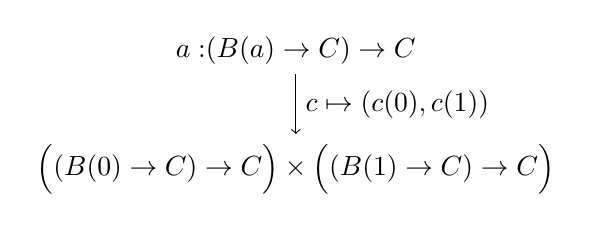
\begin{tikzpicture}
\node (N0) at (0,12) {$\prd{a:\Bool} (B(a) \to C) \to C$};
\node (N1) at (0,10.5) {$\Big((B(0) \to C) \to C\Big) \times \Big((B(1) \to C) \to C\Big)$};
\draw[->] (N0) -- node[right]{$c \mapsto (c(0), c(1))$} (N1);
\end{tikzpicture}
\end{center}
Since $B(0) = 0$, the type $B(0) \to C$ is contractible, with center $\lam{b:B(0)} \abort(C,F \; b)$. We thus have an equivalence
\begin{center}
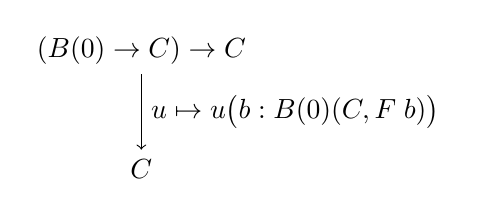
\begin{tikzpicture}
\node (N0) at (0,12) {$(B(0) \to C) \to C$};
\node (N1) at (0,10.5) {$C$};
\draw[->] (N0) -- node[right]{$u \mapsto u\big(\lam{b:B(0)} \abort(C,F \; b)\big)$} (N1);
\end{tikzpicture}
\end{center}
Since $B(1) = 1$, the map $x \mapsto \lam{\_}\; x$ is an equivalence from $C$ to $B(1) \to C$. Thus, we have an equivalence
\begin{center}
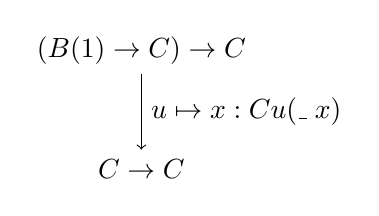
\begin{tikzpicture}
\node (N0) at (0,12) {$(B(1) \to C) \to C$};
\node (N1) at (0,10.5) {$C \to C$};
\draw[->] (N0) -- node[right]{$u \mapsto \lam{x:C} u(\lam{\_} \; x)$} (N1);
\end{tikzpicture}
\end{center}
Putting this all together, we see that the map 
\[ (C,c) \mapsto \Big(C,c\big(0,\lam{b} \abort(C,F \; b)\big),\lam{x:C} c(1, \lam{\_} \; x)\Big)\] 
is an equivalence from $\WAlg_{\UU_i}(A,B)$ to $\NatAlg_{\UU_i}$.
\end{proof}

\begin{lemma}
For any $\X : \WAlg_{\UU_i}(A,B)$ there is an equivalence
\[ \WFibAlgToNatFibAlg_{\UU_j} : \WFibAlg_{\UU_j}(A,B) \; \X \to \NatFibAlg_{\UU_j}(\WAlgToNatAlg_{\UU_i}(\X)) \]
\end{lemma}
\begin{proof}
Let an algebra $(C,c) : \WAlg_{\UU_i}(A,B)$ be given and fix $E : C \to \UU_j$. We have an equivalence
\begin{center}
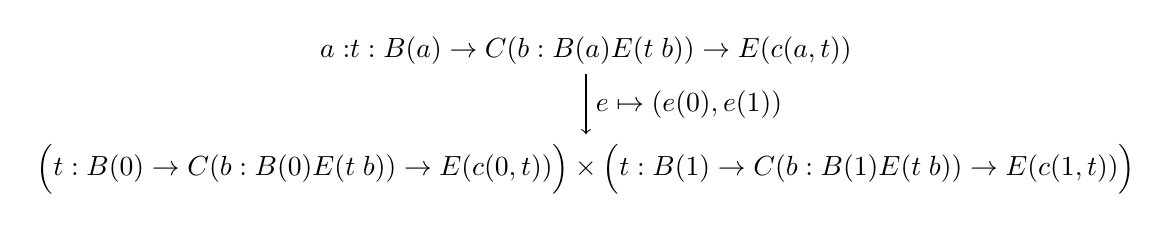
\begin{tikzpicture}
\node (N0) at (0,12) {$\prd{a:\Bool}\prd{t:B(a)\to C} (\prd{b:B(a)} E(t\;b)) \to E(c(a,t))$};
\node (N1) at (0,10.5) {$\Big(\prd{t:B(0)\to C} (\prd{b:B(0)} E(t\;b)) \to E(c(0,t))\Big) \times \Big(\prd{t:B(1)\to C} (\prd{b:B(1)} E(t\;b)) \to E(c(1,t))\Big)$};
\draw[->] (N0) -- node[right]{$e \mapsto (e(0), e(1))$} (N1);
\end{tikzpicture}
\end{center}
Since $B(0) = 0$, the type $B(0) \to C$ is contractible, with center $\lam{b:B(0)} \abort(C,F \; b)$. Likewise, $\prd{b:B(0)} E(\abort(C,F \; b))$ is contractible, with center 
$\lam{b:B(0)} \abort\big(E(\abort(C,F \; b)), F \;b\big)$. We thus have equivalences
\begin{center}
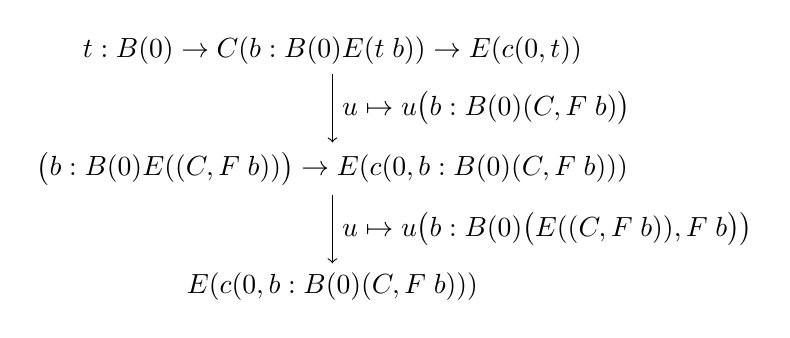
\begin{tikzpicture}
\node (N0) at (0,12) {$\prd{t:B(0)\to C} (\prd{b:B(0)} E(t\;b)) \to E(c(0,t))$};
\node (N1) at (0,10.5) {$\big(\prd{b:B(0)} E(\abort(C,F \; b))\big) \to E(c(0,\lam{b:B(0)} \abort(C,F \; b)))$};
\node (N2) at (0,9) {$E(c(0,\lam{b:B(0)} \abort(C,F \; b)))$};
\draw[->] (N0) -- node[right]{$u \mapsto u\big(\lam{b:B(0)} \abort(C,F \; b)\big)$} (N1);
\draw[->] (N1) -- node[right]{$u \mapsto u\big(\lam{b:B(0)} \abort\big(E(\abort(C,F \; b)), F \;b\big)\big)$} (N2);
\end{tikzpicture}
\end{center}
Since $B(1) = 1$, the map $x \mapsto \lam{\_}\; x$ is an equivalence from $C$ to $B(1) \to C$. Likewise, for any $x:C$ the map $y \mapsto \lam{\_}\; y$  is an equivalence from $E(x)$ to $B(1) \to E(x)$. Thus, we have equivalences
\begin{center}
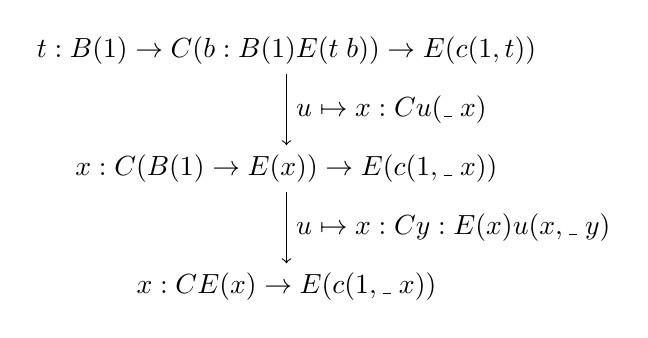
\begin{tikzpicture}
\node (N0) at (0,12) {$\prd{t:B(1)\to C} (\prd{b:B(1)} E(t\;b)) \to E(c(1,t))$};
\node (N1) at (0,10.5) {$\prd{x:C} (B(1) \to E(x)) \to E(c(1,\lam{\_} \; x))$};
\node (N2) at (0,9) {$\prd{x:C} E(x) \to E(c(1,\lam{\_} \; x))$};
\draw[->] (N0) -- node[right]{$u \mapsto \lam{x:C} u(\lam{\_} \; x)$} (N1);
\draw[->] (N1) -- node[right]{$u \mapsto \lam{x:C} \lam{y:E(x)} u(x,\lam{\_} \; y)$} (N2);
\end{tikzpicture}
\end{center}
Putting this all together, we see that the map 
\[ (E,e) \mapsto \Big(E,e\big(0,\lam{b} \abort(C,F \; b), \lam{b} \abort(E(\abort(C,F \; b)), F \;b)\big),\lam{x:C} \lam{y:E(x)} e(1, \lam{\_} \; x, \lam{\_} \; y)\Big)\] 
is an equivalence from $\WFibAlg_{\UU_j}(A,B) \; (C,c)$ to $\NatFibAlg_{\UU_j}(\WAlgToNatAlg_{\UU_i} \; (C,c))$.
\end{proof}

\begin{lemma}
For any $\X : \WAlg_{\UU_i}(A,B)$ and $\Y : \WFibAlg_{\UU_j}(A,B) \; \X$ we have
\[ \WFibHom \; \X \; \Y \;\; \simeq \;\; \NatFibHom \; \big(\WAlgToNatAlg_{\UU_i}(\X)\big) \; \big(\WFibAlgToNatFibAlg_{\UU_j}(\Y)\big) \]
\end{lemma}
\begin{proof}
Let algebras $(C,c) : \WAlg_{\UU_i}(A,B)$ and $(E,e) : \WFibAlg_{\UU_j}(A,B) \; (C,c)$ be given and fix $f : \prd{x:C} E(x)$. We have an equivalence
\begin{center}
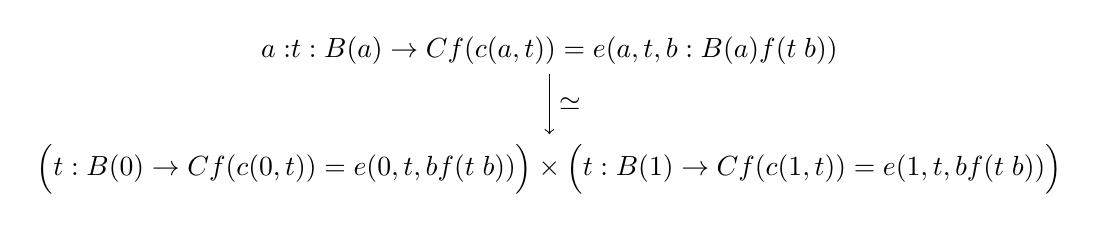
\begin{tikzpicture}
\node (N0) at (0,12) {$\prd{a:\Bool}\prd{t:B(a)\to C} f(c(a,t)) = e(a,t,\lam{b:B(a)} f(t\;b))$};
\node (N1) at (0,10.5) {$\Big(\prd{t:B(0)\to C} f(c(0,t)) = e(0,t,\lam{b} f(t\;b))\Big) \times \Big(\prd{t:B(1)\to C} f(c(1,t)) = e(1,t,\lam{b} f(t\;b))\Big)$};
\draw[->] (N0) -- node[right]{$\simeq$} (N1);
\end{tikzpicture}
\end{center}
Since $B(0) = 0$, the type $B(0) \to C$ is contractible, with center $\lam{b:B(0)} \abort(C,F \; b)$. Furthermore, since all functions out of $\zero$ are equal, we have
\[\lam{b} f(\abort(C,F \; b)) = \lam{b} \abort(E(\abort(C,F \; b)), F \;b)\] This implies the following equivalences:
\begin{center}
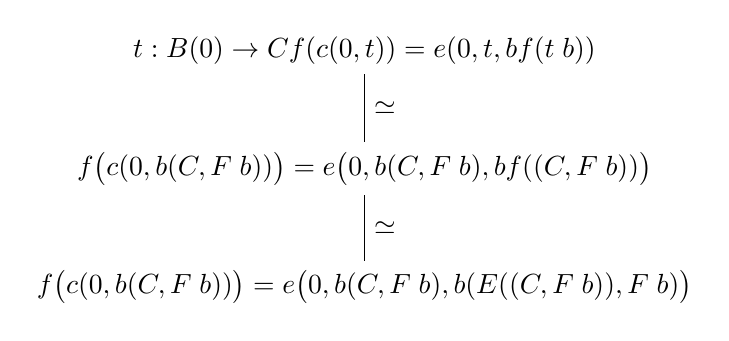
\begin{tikzpicture}
\node (N0) at (0,12) {$\prd{t:B(0)\to C} f(c(0,t)) = e(0,t,\lam{b} f(t\;b))$};
\node (N1) at (0,10.5) {$f\big(c(0,\lam{b} \abort(C,F \; b))\big) = e\big(0,\lam{b} \abort(C,F \; b),\lam{b} f(\abort(C,F \; b))\big)$};
\node (N2) at (0,9) {$f\big(c(0,\lam{b} \abort(C,F \; b))\big) = e\big(0,\lam{b} \abort(C,F \; b),\lam{b} \abort(E(\abort(C,F \; b)), F \;b)\big)$};
\draw[-] (N0) -- node[right]{$\simeq$} (N1);
\draw[-] (N1) -- node[right]{$\simeq$} (N2);
\end{tikzpicture}
\end{center}
Since $B(1) = 1$, the map $x \mapsto \lam{\_}\; x$ is an equivalence from $C$ to $B(1) \to C$. Thus, we have an equivalence
\begin{center}
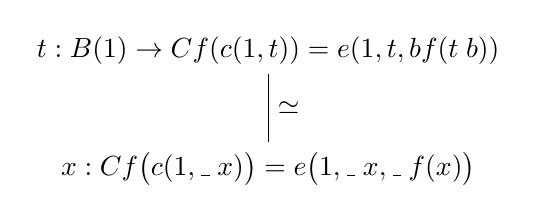
\begin{tikzpicture}
\node (N0) at (0,12) {$\prd{t:B(1)\to C} f(c(1,t)) = e(1,t,\lam{b} f(t\;b))$};
\node (N1) at (0,10.5) {$\prd{x:C} f\big(c(1,\lam{\_} \; x)\big) = e\big(1,\lam{\_} \; x,\lam{\_} \; f(x)\big)$};
\draw[-] (N0) -- node[right]{$\simeq$} (N1);
\end{tikzpicture}
\end{center}
This finishes the proof.
\end{proof}

\begin{corollary}
For any $\X : \WAlg_{\UU_i}(A,B)$ and $\Y : \WAlg_{\UU_j}(A,B)$ we have
\[ \WHom \; \X \; \Y \;\; \simeq \;\; \NatHom \; \big(\WAlgToNatAlg_{\UU_i}(\X)\big) \; \big(\WAlgToNatAlg_{\UU_j}(\Y)\big) \]
\end{corollary}

\begin{corollary}
For any $\X : \NatAlg_{\UU_i}$ we have
\begin{alignat*}{4}
& \HasNatRec_{\UU_j}(\X) & \;\; \simeq \;\; & \HasWRec_{\UU_j}(\WAlgToNatAlg_{\UU_i}^{-1}(\X)) \\
& \HasNatInd_{\UU_j}(\X) & \;\; \simeq \;\; & \HasWInd_{\UU_j}(\WAlgToNatAlg_{\UU_i}^{-1}(\X)) \\
& \HasNatRecUniq_{\UU_j}(\X) &  \simeq \;\; & \HasWRecUniq_{\UU_j}(\WAlgToNatAlg_{\UU_i}^{-1}(\X)) \\
& \HasNatIndUniq_{\UU_j}(\X) & \simeq \;\; &  \HasWIndUniq_{\UU_j}(\WAlgToNatAlg_{\UU_i}^{-1}(\X)) \\
& \IsNatHInit_{\UU_j}(\X) & \simeq \;\; & \IsWHInit_{\UU_j}(\WAlgToNatAlg_{\UU_i}^{-1}(\X))
\end{alignat*}
\end{corollary}

\begin{corollary}\label{lem:NatMainInt}
In $\Hint$, the following conditions on an algebra $\X : \NatAlg_{\UU_i}$ are equivalent:
\begin{enumerate}
\item $\X$ satisfies the induction principle on the universe $\UU_j$
\item $\X$ satisfies the recursion and recursion uniqueness principles on the universe $\UU_j$
\item $\X$ is homotopy-initial on the universe $\UU_j$  
\end{enumerate}
for $j \geq i$. In other words, we have \[ \HasNatInd_{\UU_j}(\X)  \;\; \simeq \;\; \HasNatRec_{\UU_j}(\X) \times \HasNatRecUniq_{\UU_j}(\X) \;\; \simeq \;\; \IsNatHInit_{\UU_j}(\X) \]
provided $j \geq i$. Furthermore, all 3 conditions are mere propositions.
\end{corollary}

We can thus characterize the type $\nat$ using the universal property of initiality as follows.
\begin{corollary}\label{lem:NatInitInt}
In $\Hint$ with natural numbers, the algebra $(\nat,\z,\suc(-)) : \NatAlg_{\UU_0}$ is homotopy-initial on any universe $\UU_j$.
\end{corollary}

\begin{corollary}\label{lem:NatCharInt}
In $\Hint$ extended with an algebra $\X : \NatAlg_{\UU_0}$ which is homotopy-initial on any universe $\UU_j$, the type $\nat$ with propositional computation rules is definable. 
\end{corollary}
\begin{proof}
We have an algebra $\cdot \vdash \X : \NatAlg_{\UU_0}$ such that for any $j$, there exists a term $\cdot \vdash h_j  : \IsNatHInit_{\UU_j}(\X)$. Since the requirement $j \geq 0$ always holds, Cor.~\ref{lem:NatMainInt} implies that for any $j$, we have a term $\cdot \vdash r_j : \HasNatInd_{\UU_j}(\X)$. This implies that the type $\nat$ with propositional computation rules is definable.
\end{proof}

%Finally, let us observe that the definition of a type representing the second number class as a W-type,
%as discussed in~\cite{MartinLofP:inttt}, carries over equally well. Indeed, one
%now must represent type-theoretically a signature with three operations: the first of arity zero, 
%the second of arity one, and the third of arity $\nat$. For the first two we can proceed exactly as
%before, while for the third there is no need to prove auxiliary results on adjoint homotopy 
%equivalences. As before, the second number class supports an h-initial algebra structure for the corresponding polynomial functor $P(X) = \mathsf{1} + X + (\nat \rightarrow X)$.
%Again, the formal development of this result in Coq can be found in~\cite{AwodeyS:indtht}.

%Finally, the case $\List(A)$ of finite lists of elements of type $A$ can be treated analogously, in terms of the polynomial functor 
%\[
%P(X) = \mathsf{1} + A\!\times\! X\, .
%\]
%%
%We again refer to~\cite{AwodeyS:indtht} for details.
